\documentclass[5p,times]{elsarticle}

% Math and symbols
\usepackage{amsmath,amssymb,amsfonts}
\usepackage{bm}

% Figures and tables
\usepackage{graphicx}
\usepackage{booktabs}
\usepackage{multirow}
\usepackage{subfig}
\usepackage{array}
\usepackage{float}

% Colors and links
\usepackage{xcolor}
\usepackage{hyperref}
\hypersetup{
    colorlinks=true,
    linkcolor=blue,
    filecolor=magenta,
    urlcolor=cyan,
    citecolor=blue
}

% Algorithms
\usepackage{algorithm}
\usepackage{algorithmic}
\floatname{algorithm}{Algorithm}
\renewcommand{\algorithmicrequire}{\textbf{Input:}}
\renewcommand{\algorithmicensure}{\textbf{Output:}}

% Code
\usepackage{listings}

% Others
\usepackage{url}
\usepackage{enumitem}
\usepackage{threeparttable}

% Image path
\graphicspath{{figures/}}

\begin{document}

\begin{frontmatter}

\title{Comparative Study of Missing Indicator-Based State of Health Prediction for Lithium-Ion Batteries: Deep Learning Models and Multi-Missing-Rate Experiments on XJTU Dataset}

\author[inst1]{Qingyang Chen}
\ead{202414544@mail.sdu.edu.cn}
\author[inst1]{Qiang Zhang\corref{cor1}}
\ead{sduzhangqiang@sdu.edu.cn}
\author[inst2]{Yunfei Wang}
\cortext[cor1]{Corresponding author.}

\address[inst1]{School of Nuclear Science and Energy Engineering, Shandong University, Jinan 250061, China}
\address[inst2]{Shandong Supermaly Generating Equipment Co., Ltd, No.5153 Yingqian Street, Hi-technology Development Zone, Weifang 261061, Shandong, China}

\begin{abstract}
Accurate State of Health (SOH) estimation is essential for safe and reliable operation of electric vehicles and energy storage systems, yet sensor failures and data acquisition anomalies frequently cause missing monitoring data. Traditional methods treat missing values as noise, neglecting the information contained in the pattern of missingness itself, which limits performance at high missing rates. Using the public XJTU lithium-ion battery dataset, we introduce a simple Missing Indicator Matrix (MIM) approach and systematically evaluate its impact on SOH prediction across four deep learning architectures---MLP, LSTM, GRU, and 1D-CNN---under varying missing-rate conditions. Results demonstrate that for missing rates $\geq$0.4, MIM consistently improves prediction accuracy, reducing error by 26--57\% across all models compared to imputation-only baselines. The improvement is observed uniformly across architectures, indicating that the missing-indicator signal is more valuable than the imputation method itself. This study provides a concise, effective technical solution for handling missing data in Battery Management Systems, enhancing the practicality and reliability of data-driven SOH prediction methods in real-world engineering applications.
\end{abstract}

\begin{keyword}
lithium-ion battery \sep State of Health (SOH) prediction \sep missing data \sep Missing Indicator Matrix (MIM) \sep XJTU dataset \sep deep learning
\end{keyword}

\end{frontmatter}

%==============================================================================
\section{Introduction}\label{sec:intro}

\subsection{Energy System Background and Data Missing Pain Points}

Against the backdrop of global energy structure transformation and rapid development of transportation electrification, lithium-ion batteries, as key energy storage units, have been deployed at large scale in electric vehicles, grid-scale energy storage, and distributed energy systems. Accurate estimation and prediction of battery State of Health (SOH) is a core link for ensuring system operational safety, optimizing energy management strategies, and controlling full lifecycle costs. In large-scale electric vehicle fleets and grid-scale energy storage systems, SOH estimation accuracy directly affects capacity planning and dispatch strategies, serving as an important foundation for ensuring high penetration of renewable energy sources.

In recent years, data-driven SOH prediction methods have received widespread attention\cite{luo2022review}. These methods learn complex nonlinear mapping relationships between features and SOH from historical operational data, avoiding the construction and identification of complex electrochemical mechanism models, and demonstrating clear advantages in adaptability and scalability. From shallow models to deep neural architectures such as MLP, CNN, and RNN/LSTM/GRU, various algorithms have continuously improved prediction accuracy on publicly available benchmark datasets\cite{liu2025deep}, laying a solid foundation for the engineering application of SOH prediction.

However, in practical engineering scenarios, sensor data collected by Battery Management Systems (BMS) often suffers from varying degrees of missing data. The main causes of data missing can be categorized into three types: \textbf{(1) Sensor failures and aging} leading to measurement failures; \textbf{(2) Unstable communication links} causing data packet loss; \textbf{(3) Sampling strategy optimization or protection mechanism triggering} leading to intermittent recording interruptions. In large-scale energy storage stations or fleet-level application scenarios, this problem is particularly prominent due to the large number of batteries and dense monitoring points.

When input features exhibit significant missing data, traditional data-driven models often face issues such as inconsistent input dimensions, feature distribution shifts, and increased prediction uncertainty; in extreme cases, model outputs may become distorted or even completely fail. Figure~\ref{fig:problem_scenario} illustrates the BMS monitoring chain and the corresponding cycle-level feature matrix, where multi-source failures lead to random missing patterns in the feature matrix. In current practice, these missing problems are often addressed through data screening or conservative strategies, resulting in substantial reduction of available samples and making SOH prediction models difficult to generalize to real-world complex operating conditions.

\begin{figure*}[t]
    \centering
    
\includegraphics[width=\textwidth]{fig1_problem_scenario.png}
    \caption{Schematic diagram of data missing problems in battery SOH prediction. (a) BMS monitoring chain and potential failure sources; (b) Cycle-level feature matrix and MCAR missing patterns.}
    \label{fig:problem_scenario}
\end{figure*}

\subsection{Limitations of Existing SOH Prediction and Missing Data Treatment}

Regarding missing data problems in BMS monitoring data, existing research roughly adopts three categories of treatment strategies: deletion methods, imputation methods, and model-based methods.

\textbf{Deletion methods} avoid processing missing values themselves by directly discarding samples or features containing missing values, but in high missing rate scenarios, this causes severe information loss and selection bias, making it difficult to meet the data utilization requirements of energy systems.

\textbf{Imputation methods} estimate and fill missing values through statistics (mean, median) or prediction models (K-nearest neighbors, regression, etc.), and are currently the most widely used in industry. However, such methods struggle to characterize the uncertainty introduced by missing data and cannot explicitly encode the potentially useful information of ``which features are missing where.''

\textbf{Model-based methods} (such as multiple imputation, probabilistic graphical models, etc.) are theoretically more rigorous, but often require complex distribution assumptions, with high computational costs and implementation difficulties, making direct deployment difficult in resource-constrained BMS environments with high real-time requirements.

The above traditional methods generally follow the ``repair data first, then predict'' processing paradigm, treating missing data as noise to be eliminated rather than potential health state indicator signals. In engineering practice, this paradigm often forces BMS to adopt overly conservative energy management strategies, thereby increasing system redundancy and operational costs. During battery aging processes, certain sensor channels are more prone to anomalies or failures under high-temperature, high-load conditions, making missing patterns potentially correlated with SOH, which traditional methods cannot exploit.

\subsection{Core Paradigm: Missing as Signal}

Addressing the mainstream treatment approach that generally regards missing data as noise, this paper proposes the ``missing as signal'' modeling paradigm in the battery SOH prediction task, treating missing patterns themselves as first-order input features to be utilized. This paper introduces and systematically evaluates a simple and easily engineering-implementable missing data treatment strategy---the Missing Indicator Matrix (MIM) method\cite{jones1996indicator,van2023missing}. This method constructs corresponding binary indicator variables for each potentially missing feature on top of conventional imputation and feeds them into the prediction model together with the imputed features.

From a modeling paradigm perspective, traditional methods follow the two-stage ``impute first, then predict'' workflow:
\begin{equation}
    \text{Impute}(X) \rightarrow \text{Predict}(Y)
\end{equation}
In this workflow, missing indicator information is eliminated during the imputation stage. In contrast, the MIM method adopts an end-to-end joint learning paradigm:
\begin{equation}
    \text{Predict}(Y \mid X_{\mathrm{obs}}, M)
\end{equation}
where $X_{\mathrm{obs}}$ represents observed feature values and $M$ represents the missing indicator matrix. In the traditional $\text{Impute}(X)\rightarrow\text{Predict}(Y)$ workflow, missing indicator information $M$ is eliminated before imputation; while under the $\text{Predict}(Y \mid X_{\mathrm{obs}}, M)$ paradigm, the model can simultaneously utilize real observations $X_{\mathrm{obs}}$ and missing patterns $M$, avoiding critical information loss. Unlike traditional approaches that focus solely on ``filling in missing values,'' MIM emphasizes explicitly encoding ``which values are missing'' and allowing the model to learn the joint effects of feature values and missing patterns on SOH during training.

Previous research has shown that when missing patterns are informative, MIM can significantly improve prediction performance in medical data analysis, recommendation systems, and other domains\cite{sisk2023imputation,ehrig2025imputation}. In large-scale fleet and grid-scale energy storage systems, sampling strategies are dynamically adjusted according to operating conditions, and sensor aging patterns are often related to degradation processes; these characteristics make the ``missing as signal'' modeling paradigm naturally applicable in energy applications. This paper will verify the effectiveness of the MIM method in battery SOH prediction tasks through a series of well-controlled experiments based on the publicly available XJTU lithium-ion battery dataset, and provide quantitative references for handling missing data in engineering practice.

\subsection{Main Innovations and Contributions}

To systematically evaluate the role of the Missing Indicator Matrix method in battery SOH prediction, this paper focuses on three questions: first, under different Missing Rates (MR), what magnitude of performance and stability benefits can MIM bring relative to imputation-only schemes; second, among typical deep architectures such as MLP, LSTM, GRU, and 1D-CNN, whether there are significant differences in MIM benefits; third, under extreme high missing rate conditions, which ``model + MIM'' combinations can still maintain acceptable SOH prediction accuracy and robustness.

Centered around the above research questions, this paper conducts work from three levels: methodological paradigm, empirical framework, and engineering application. The core innovations are summarized as follows:

\begin{itemize}
  \item \textbf{Paradigm innovation: repositioning ``missing patterns'' as first-order input features.} In the battery SOH prediction task, the ``missing as signal'' modeling paradigm is systematically proposed and validated, shifting from the traditional $\text{Impute}(X)\rightarrow\text{Predict}(Y)$ to $\text{Predict}(Y \mid X_{\mathrm{obs}}, M)$, avoiding the elimination of information carried by missing patterns during the preprocessing stage.

  \item \textbf{Experimental framework innovation: constructing a unified evaluation benchmark for multi-missing-rate, multi-architecture scenarios.} Based on the XJTU publicly available battery dataset, an experimental framework covering nine levels of missing rates (MR=0.1--0.9), four typical deep learning architectures (MLP, LSTM, GRU, 1D-CNN), and 100 random seeds was designed. Under unified preprocessing and training configurations, the performance benefits and statistical significance of MIM were systematically evaluated through Wilcoxon signed-rank tests.

  \item \textbf{Training strategy innovation: proposing multi-missing-rate joint training to enhance robustness.} By explicitly mixing samples with various missing rates during the training stage, a multi-missing-rate joint training strategy is proposed, enabling a single MIM model to maintain robust performance when facing unknown missing patterns, providing methodological support for deploying SOH prediction under complex operating conditions.

  \item \textbf{Engineering value innovation: providing BMS model selection recommendations for different missing rate intervals.} Systematic trade-offs among error, parameter count, and missing rate are conducted to construct quantitative mapping relationships of ``missing rate interval---model architecture---MIM usage,'' providing actionable algorithm selection guidelines for BMS design in electric vehicles and energy storage systems.
\end{itemize}

\subsection{Paper Organization}

The remainder of this paper is organized as follows: Section~\ref{sec:related} reviews research on lithium battery SOH prediction methods and missing data treatment with MIM; Section~\ref{sec:method} presents the MIM input strategy and model framework of this paper, including sample construction, missing simulation, and multi-missing-rate joint training strategy; Section~\ref{sec:results} presents experimental settings and comparative results under multi-missing-rate conditions on the XJTU dataset; Section~\ref{sec:discussion} discusses the mechanism of MIM and engineering application scenarios, and provides model selection recommendations for BMS; Section~\ref{sec:conclusion} summarizes the work and its potential impact on energy systems, and outlines future research directions.

%==============================================================================
\section{Related Work and Technical Background}\label{sec:related}

\subsection{Battery SOH Estimation: From Physical Models to Deep Learning}

In electric vehicle fleets and grid-scale energy storage systems, accurate estimation of battery SOH is directly related to system safety, economy, and lifetime management. Battery SOH prediction, as a typical regression problem, has evolved from physics-based to data-driven modeling approaches. Early physics-based methods described internal battery aging mechanisms through electrochemical impedance spectroscopy and equivalent circuit models\cite{wang2020phys,yang2019ecm}, offering clear physical interpretability, but with numerous model parameters that are difficult to identify, and poor adaptability to different chemistries and operating conditions. With the development of machine learning technology, data-driven methods have gradually become mainstream\cite{liu2025deep,shao2023review,wang2023battery}, which can be roughly divided into three categories based on model structural characteristics: feedforward networks (MLP), recurrent neural networks (LSTM/GRU), and one-dimensional convolutional neural networks (1D-CNN).

Multilayer Perceptron (MLP), as the most basic neural network structure, learns complex mapping relationships between features and SOH through multi-layer nonlinear transformations, featuring simple structure and controllable parameter count, making it suitable as a baseline method and for resource-constrained scenarios\cite{bairwa2025cycle}. Temporal models, represented by LSTM and GRU, can explicitly model temporal dependencies between adjacent cycles in terms of capacity and features, utilizing historical information to assist current prediction\cite{hochreiter1997lstm,cho2014gru}, demonstrating better stability in complex situations such as capacity regeneration and aging trend turning points. One-dimensional convolutional neural networks (1D-CNN) extract local feature patterns along the temporal dimension through convolution kernels, featuring high parallel computational efficiency and strong local pattern recognition capabilities\cite{lecun2015cnn}, performing excellently under conditions with relatively limited training data\cite{zhang2024cnnsoh}. The above three architectures each have advantages in capturing temporal dependencies and cross-cycle features, and have been widely used for battery SOH prediction and remaining useful life estimation tasks on unified datasets\cite{bairwa2025cycle}.

It is worth noting that most existing SOH prediction research assumes that input data is essentially complete, with less systematic consideration of data missing problems\cite{shao2025soh,deng2025novel}. Early research mainly focused on feature engineering and model construction under standard operating conditions and complete data conditions. Typical electrical signal feature modeling methods include Independent Component Analysis (ICA), Differential Voltage Analysis (DVA), etc., used to extract key features characterizing aging degree from voltage and current curves\cite{deng2025novel}. These methods can achieve high prediction accuracy when data is complete, but have strong dependence on data integrity, making it difficult to directly migrate to practical operating scenarios with widespread missing data. The above methods and feature engineering techniques perform well when data is complete, but are naturally fragile to missing data, which urgently demands subsequent research on missing data treatment methods.

\subsection{Missing Data Theory and Missing Indicator Matrix (MIM)}

In practical data analysis tasks, data missing is a ubiquitous challenge. From a statistical perspective, missing mechanisms are typically classified into three categories: missing completely at random (MCAR), where missingness is unrelated to any observed or unobserved variables; missing at random (MAR), where missingness can be explained by observed variables; and missing not at random (MNAR), where missingness is related to the unobserved variable values themselves\cite{little2002statistical,rubin1976inference}. Under different missing mechanisms, appropriate treatment strategies also vary.

Traditional missing data treatment methods can be mainly categorized into three types: deletion methods, single-value imputation methods, and model-based methods. Deletion methods are simple and effective when the Missing Rate (MR) is low, but at high missing rates, they lose substantial information and may introduce selection bias. Single-value imputation methods (such as mean imputation, regression imputation, etc.) preserve sample size but underestimate variance and distort relationships between variables. Model-based methods such as Expectation-Maximization (EM) algorithms and Multiple Imputation handle missing data by establishing probabilistic models, which are theoretically more rigorous but computationally complex, usually requiring certain assumptions about data distributions or missing mechanisms.

The Missing Indicator Matrix (MIM) method provides a modeling approach distinct from traditional deletion and imputation strategies\cite{jones1996indicator,van2023missing}. The core idea of this method is to explicitly encode missing information as additional binary features, feeding them into the model together with original features, allowing the model to learn how to utilize missing pattern information during training\cite{ipsen2022deal}. Specifically, for each feature that may have missing values, a corresponding indicator variable is constructed, with the indicator being 1 when the feature value is missing and 0 otherwise. Thus, the original feature vector $X$ is expanded to $[X, M]$, where $M$ is the indicator vector.

From a theoretical perspective, the effectiveness of the MIM method depends on the correlation between missing mechanisms and target variables. When missing data is missing completely at random (MCAR), indicators contain no information about the target variable, and MIM may only bring marginal improvements; but when missing data is related to the target variable (MAR or MNAR), indicators become valuable predictive signals. In battery SOH prediction scenarios, some sensors gradually fail with the aging process, or are more prone to recording interruptions under specific operating conditions such as high temperature and high rates, making missing patterns themselves correlated with SOH and thus possessing potential for MIM utilization. Therefore, missing patterns themselves can be regarded as indirect observations about SOH, having potential value in both theoretical analysis and engineering applications.

The MIM method has been successfully applied in multiple domains. In medical data analysis, due to the selective nature of patient examination items, electronic medical record data commonly suffers from structural missing data; research has shown that introducing missing indicators can significantly improve disease prediction model performance\cite{sisk2023imputation,ehrig2025imputation}. In recommendation systems and time series modeling, work has also adopted feature masking or missing indicator vectors to explicitly model missing patterns, achieving performance improvements\cite{ipsen2022deal,che2018recurrent}. However, systematic evaluation of explicit missing modeling represented by MIM in battery SOH prediction tasks remains scarce, lacking comparative conclusions under unified datasets and multi-missing-rate conditions. Particularly in battery SOH prediction, a complex engineering problem with strong temporal characteristics and multi-physics coupling, systematic research on the MIM method remains a gap, and its applicability and actual benefits under different deep learning architectures have not been fully verified. This constitutes one of the core motivations for the empirical research conducted in this paper.

\subsection{Battery Datasets and Missing-Data Issues in BMS}

In recent years, multiple open battery datasets have been released to support SOH prediction research, including NASA, CALCE, Oxford, and XJTU datasets\cite{severson2019data,wang2024open,duan2025lithium,wang2024pinn}. Among them, the XJTU dataset adopted in this study contains cycling aging data of various mainstream chemistries (LFP, NMC) under different charge-discharge conditions, providing high-quality benchmark data for evaluating missing data treatment methods.

Despite the availability of rich datasets, most existing SOH prediction research assumes that input data is essentially complete, with less systematic consideration of data missing problems\cite{shao2025soh,deng2025novel,chen2024batteryMissing}. While some studies have explored imputation methods for battery sensor data\cite{li2023bmsImputation}, the approach of explicitly encoding missing patterns as predictive signals (MIM) remains largely unexplored in battery management applications. This gap is particularly critical because BMS in electric vehicle fleets and grid-scale energy storage systems frequently encounter sensor failures and communication interruptions, making missing data a ubiquitous challenge in real-world engineering scenarios.

\subsection{Gaps in Existing Work and Positioning of This Paper}

In summary, existing research has key gaps in three areas: (1) unified evaluation frameworks covering multiple missing rates, (2) cross-architecture comparisons of MIM effects, and (3) publicly available experiments with strictly controlled variables. Filling these gaps helps clarify the real benefits and applicable boundaries of MIM in battery SOH prediction.

Compared with existing literature, this research distinguishes itself in three aspects. First, it treats missing data treatment as core research content rather than a preprocessing afterthought. Second, it adopts the MIM approach of encoding missing information explicitly, rather than focusing solely on improving imputation accuracy. Finally, it covers nine levels of missing rates (MR=0.1--0.9) for comprehensive evaluation, whereas existing research usually validates methods only under single or few missing rates.

%==============================================================================
\section{Methodology: MIM Input Strategy and Model Framework}\label{sec:method}

\subsection{Problem Definition and Notation}

This study adopts the publicly available XJTU lithium-ion battery dataset from Xi'an Jiaotong University as the experimental platform\cite{wang2024open,duan2025lithium}. This dataset contains cycling aging data of various mainstream chemistries (such as LFP, NMC) under different charge-discharge conditions, covering multiple rate and operating condition batches, providing high-quality benchmark data for SOH prediction research\cite{wang2024open,wang2024pinn}.

In terms of sample construction, this study builds samples with cycles as the basic unit. For each charge-discharge cycle, a corresponding 16-dimensional statistical feature vector is extracted as input, and the ratio of the measured discharge capacity of that cycle to the initial capacity is used as the SOH label:
\begin{equation}
    \text{SOH}_t = \frac{Q_t}{Q_0} \times 100\%
    \label{eq:soh}
\end{equation}
where $Q_t$ is the measured discharge capacity of the $t$-th cycle and $Q_0$ is the initial rated capacity. Using relative capacity (SOH) eliminates the influence of different initial capacities among batteries.

The Missing Rate (MR) is defined as the proportion of missing elements in the feature matrix to the total elements:
\begin{equation}
    \text{MR} = \frac{1}{n \times d} \sum_{i=1}^{n}\sum_{j=1}^{d} \mathbb{I}(x_{ij}\ \text{missing})
    \label{eq:mr}
\end{equation}
where $n$ is the number of samples, $d=16$ is the feature dimension, and $\mathbb{I}(\cdot)$ is the indicator function. This cycle-level SOH modeling approach is consistent with the actual operation mode of BMS in electric vehicle fleets and grid-scale energy storage systems, both estimating current battery health status based on monitoring data from single charge-discharge cycles, laying a good foundation for subsequent method migration and application in real scenarios.

\subsection{Sample Construction and Feature Engineering}

After data cleaning, the dataset retains approximately 9,000 valid cycle samples, covering the complete aging process from initial state to SOH dropping to approximately 50\%. This study constructs 16-dimensional cycle-level statistical features from three dimensions: voltage, current, and charging process:

\textbf{Voltage statistical features} (4 dimensions): mean, standard deviation, skewness, and kurtosis, used to characterize the overall morphology of voltage distribution, reflecting changes in battery internal resistance and polarization characteristics.

\textbf{Charging process features} (4 dimensions): constant-current phase charging capacity and time, voltage slope and voltage entropy, reflecting battery charging acceptance capability and voltage signal complexity.

\textbf{Current statistical features} (8 dimensions): mean, standard deviation, skewness, and kurtosis, as well as constant-voltage phase charging capacity, time, current slope, and current entropy, characterizing current fluctuation characteristics and constant-voltage phase decay behavior.

All features undergo Z-score standardization before being fed into the model, with standardization parameters (mean $\mu_j$, standard deviation $\sigma_j$) calculated only on the training set to ensure independence of data partitioning:
\begin{equation}
    z_{ij} = \frac{x_{ij} - \mu_j}{\sigma_j}
\end{equation}

Data preprocessing includes three steps: \textbf{(1) Outlier removal}, eliminating abnormal cycles with SOH$>$100\% or SOH$<$50\%; \textbf{(2) Noise smoothing}, conducting anomaly detection and smoothing for continuous features such as voltage and current; \textbf{(3) Sequence alignment}, ensuring cycle sequence continuity and completeness, avoiding temporal discontinuities.

\subsection{Missing Simulation, Imputation, and MIM Construction}

To systematically evaluate model performance under different Missing Rate (MR) conditions, this study adopts the missing completely at random (MCAR) mechanism, injecting nine levels of missing rates $\{0.1, 0.2, \ldots, 0.9\}$ at the feature level. Under the MCAR mechanism, the selection of missing positions is unrelated to feature values, SOH labels, etc., facilitating controlled experimental conditions and constituting a baseline scenario for evaluating method robustness to missing data.

In terms of imputation strategy, this study adopts mean imputation as the unified baseline. For missing values, the mean of the corresponding feature on the training set is used for filling:
\begin{equation}
    \hat{x}_{ij} = \begin{cases}
        x_{ij}, & \text{if } x_{ij} \text{ observed} \\
        \bar{x}_j, & \text{if } x_{ij} \text{ missing}
    \end{cases}
\end{equation}
This method has low computational cost, is easy to implement, and as a widely used simple imputation scheme, provides a fair comparison baseline for evaluating the gains brought by MIM.

MIM is the core method of this study. For each original feature, a corresponding binary missing indicator variable is constructed:
\begin{equation}
    m_{ij} = 
    \begin{cases}
        0, & \text{if } x_{ij} \text{ observed} \\
        1, & \text{if } x_{ij} \text{ missing}
    \end{cases}
\end{equation}

Based on the above definitions, two input representation strategies are constructed: \textbf{Baseline strategy} uses only the imputed feature vector $\hat{X} \in \mathbb{R}^{n \times 16}$; \textbf{MIM strategy} concatenates imputed features with missing indicators, forming an extended input $[\hat{X} \,|\, M] \in \mathbb{R}^{n \times 32}$, allowing the model to simultaneously utilize feature value and missing pattern information.

Algorithm~\ref{alg:mim} presents the high-level process of MIM construction:

\begin{algorithm}[t]
\caption{Missing Indicator Construction and Input Representation Generation}
\label{alg:mim}
\begin{algorithmic}[1]
\REQUIRE Raw feature matrix $X \in \mathbb{R}^{n \times d}$, missing rate $p \in [0, 1]$
\ENSURE Imputed features $\hat{X}$, missing indicators $M$, extended input $Z = [\hat{X} \,|\, M]$
\STATE Sample missing mask according to MCAR mechanism: $\Omega_{ij} \sim \text{Bernoulli}(1-p)$
\STATE Construct missing indicator matrix: $M_{ij} = \mathbf{1}(\Omega_{ij} = 0)$
\STATE Mean imputation: $\hat{X}_{ij} = \bar{x}_j$ (if $\Omega_{ij}=0$), otherwise $\hat{X}_{ij} = X_{ij}$
\STATE Concatenate extended input: $Z = [\hat{X} \,|\, M]$
\STATE \textbf{return} $\hat{X}$, $M$, $Z$
\end{algorithmic}
\end{algorithm}

Figure~\ref{fig:baseline_vs_mim} visually demonstrates the comparison between the two input strategies.

\begin{figure}[t]
    \centering
    
\includegraphics[width=\columnwidth]{fig2_baseline_vs_mim.png}
    \caption{Comparison of Baseline and MIM input strategies. (a) Baseline: 16-dimensional imputed features $\hat{X}$; (b) MIM: concatenated 32-dimensional extended input $[\hat{X} \,|\, M]$.}
    \label{fig:baseline_vs_mim}
\end{figure}

\subsection{Deep Learning Model Architectures and Parameter Configuration}

To ensure fairness in experimental comparisons, this study controls the parameter counts of the four models to the same order of magnitude of approximately 15k--45k, making comparisons focus more on input forms (Baseline vs. MIM) rather than model capacity differences. Based on architecture search from preliminary experiments, the optimal configurations for each model are determined as follows:

\textbf{MLP}: Four hidden layers (192$\rightarrow$96$\rightarrow$48$\rightarrow$24), ReLU activation, Dropout=0.15.

\textbf{LSTM}: Two-layer recurrent structure, 48 hidden units, sequence length 5, Dropout=0.2.

\textbf{GRU}: Two-layer recurrent structure, 64 hidden units, sequence length 5, Dropout=0.2.

\textbf{1D-CNN}: Two convolutional layers (channels 72$\rightarrow$32), kernel size 4, adaptive pooling, Dropout=0.1.

Model architecture and parameter configurations are summarized in Table~\ref{tab:model_config}. Due to MIM input dimension increasing from 16 to 32, parameter counts increase accordingly (for example, MLP grows from 27,649 to 36,865 parameters).

\begin{table*}[t]
\centering
\small
\caption{Model Architecture and Parameter Configuration (Optimal Configurations Determined by Architecture Search)}
\label{tab:model_config}
\begin{threeparttable}
\begin{tabular}{@{}llp{4.5cm}rr@{}}
\toprule
\textbf{Model} & \textbf{Architecture Details} & \textbf{Key Hyperparameters} & \textbf{Baseline} & \textbf{MIM} \\
\midrule
MLP & Input$\rightarrow$192$\rightarrow$96$\rightarrow$48$\rightarrow$24$\rightarrow$1 & ReLU, Dropout=0.15 & 27,649 & 36,865 \\
LSTM & 2-layer LSTM$\rightarrow$FC & hidden=48, seq\_len=5, Dropout=0.2 & 31,537 & 40,753 \\
GRU & 2-layer GRU$\rightarrow$FC & hidden=64, seq\_len=5, Dropout=0.2 & 40,769 & 49,985 \\
1D-CNN & Conv1d(16$\rightarrow$72$\rightarrow$32)$\rightarrow$FC & kernel=4, Dropout=0.1 & 16,713 & 30,537 \\
\bottomrule
\end{tabular}
\begin{tablenotes}
    \item Note: Parameter counts include trainable weights and biases, controlled within the range of 15k--45k.
\end{tablenotes}
\end{threeparttable}
\end{table*}

\begin{figure*}[t]
    \centering
    
\includegraphics[width=\textwidth]{fig3_model_architectures.png}
    \caption{Comparison of four deep learning model architectures. (a) MLP; (b) LSTM; (c) GRU; (d) 1D-CNN.}
    \label{fig:model_architectures}
\end{figure*}

\subsection{Multi-Missing-Rate Joint Training Strategy}

Regarding dataset partitioning, division is performed by battery cell rather than cycle samples (training/validation/testing $\approx$ 60\%/20\%/20\%), ensuring that the testing phase evaluates ``unseen batteries'' and avoids information leakage. All models share the training configurations shown in Table~\ref{tab:training_config}.

\begin{table}[t]
\centering
\footnotesize
\caption{Training Hyperparameter Configuration}
\label{tab:training_config}
\begin{tabular}{@{}lp{2cm}p{3.5cm}@{}}
\toprule
\textbf{Hyperparameter} & \textbf{Config.} & \textbf{Description} \\
\midrule
Optimizer & Adam & Adaptive learning rate \\
Learning rate & $10^{-3}$ & Initial learning rate \\
Batch size & 32 & Mini-batch gradient descent \\
Max epochs & 200 & Max epochs before early stopping \\
Early stop patience & 15 rounds & Stop if validation loss not decrease \\
Loss function & MSE & Mean squared error \\
\bottomrule
\end{tabular}
\end{table}

\begin{table}[t]
\centering
\footnotesize
\caption{Dataset Partition Details}
\label{tab:data_split}
\begin{tabular}{@{}lcccp{2.8cm}@{}}
\toprule
\textbf{Subset} & \textbf{Prop.} & \textbf{\#Batt.} & \textbf{\#Cyc.} & \textbf{Purpose} \\
\midrule
Training & 60\% & $\approx$18 & $\approx$6,000 & Model parameter learning \\
Validation & 20\% & $\approx$6 & $\approx$2,000 & Hyperparameter tuning \\
Testing & 20\% & $\approx$6 & $\approx$2,000 & Final evaluation \\
\bottomrule
\end{tabular}
\end{table}

For MIM models, this study proposes a multi-missing-rate joint training strategy: the complete training set generates 10 copies with missing data under Missing Rates (MR) $\{0.0, 0.1, \ldots, 0.9\}$ respectively, which after MIM construction are merged into an augmented training set $\mathcal{D}_{\text{augmented}}$ expanded by 10 times. Training a unified MIM model on this augmented set allows it to encounter various typical missing patterns during the training stage, enhancing robustness to unknown missing conditions. The validation set adopts a fixed MR=0.5 for evaluating generalization performance. Baseline models are trained only on complete data (MR=0.0), as missing data in training data without missing indicators would only bring noise.

Algorithm~\ref{alg:training} describes the multi-missing-rate joint training process for MIM models:

\begin{algorithm}[t]
\caption{Multi-Missing-Rate Joint Training for MIM Models}
\label{alg:training}
\begin{algorithmic}[1]
\REQUIRE Complete training set $\mathcal{D}_{\text{train}} = \{X, Y\}$, missing rate set $\mathcal{P} = \{0.0, 0.1, \ldots, 0.9\}$
\ENSURE Trained MIM model $f_{\text{MIM}}$
\STATE Initialize augmented training set: $\mathcal{D}_{\text{augmented}} \leftarrow \emptyset$
\FOR{$p \in \mathcal{P}$}
    \STATE Call Algorithm~\ref{alg:mim} to generate: $(\hat{X}^{(p)}, M^{(p)}, Z^{(p)})$
    \STATE Merge: $\mathcal{D}_{\text{augmented}} \leftarrow \mathcal{D}_{\text{augmented}} \cup \{(Z^{(p)}, Y)\}$
\ENDFOR
\STATE Mini-batch training on $\mathcal{D}_{\text{augmented}}$, early stopping on validation set (MR=0.5)
\STATE \textbf{return} $f_{\text{MIM}}$
\end{algorithmic}
\end{algorithm}

Figure~\ref{fig:joint_training} illustrates the specific process of multi-missing-rate joint training.

\begin{figure*}[t]
    \centering
    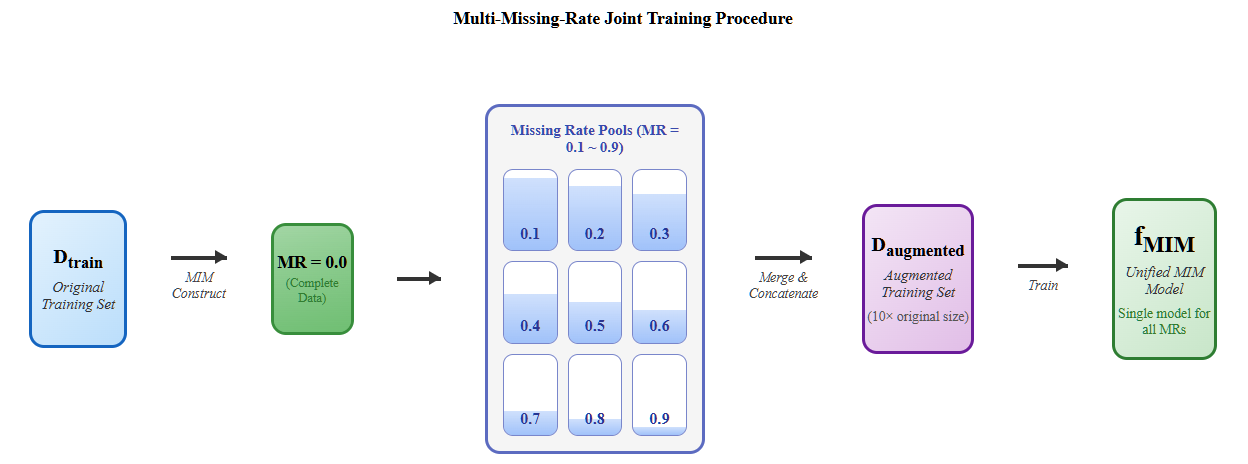
\includegraphics[width=\textwidth]{fig4_joint_training.png}
    \caption{Multi-missing-rate joint training process. The original training set generates copies at 10 missing rates, which after MIM construction are merged into $\mathcal{D}_{\text{augmented}}$ for training a unified MIM model.}
    \label{fig:joint_training}
\end{figure*}

Model performance is evaluated using three regression metrics: MAE, RMSE, and R\textsuperscript{2} (definitions in Section~\ref{sec:results}).

%==============================================================================
\section{Experimental Results and Analysis}\label{sec:results}

\subsection{Dataset and Experimental Settings}

This experiment is based on the XJTU publicly available lithium-ion battery dataset\cite{wang2024open}, containing cycling aging data of LFP, NMC, and other mainstream chemistries under different charge-discharge conditions. After data cleaning, approximately 9,000 valid cycle samples are retained, using ``cycle-level 16-dimensional features + SOH label'' as the basic modeling unit (see Section~\ref{sec:method} for details).

Data partitioning adopts division by battery cell rather than cycle samples, with data from different batteries assigned to training, validation, and testing sets respectively, with proportions of approximately 60\%/20\%/20\% (see Table~\ref{tab:data_split} for details). This partitioning strategy ensures that the testing phase evaluates ``unseen batteries,'' avoiding information leakage between different cycles of the same battery.

All models share unified training configurations (see Table~\ref{tab:training_config} for details), implemented in Python 3.12 and PyTorch 2.10.0 environment. The entire process of data partitioning, missing simulation, and model training is repeated with 100 different random seeds (42--141), reporting ``mean $\pm$ standard deviation'' as final results.

Model performance is evaluated using the following three regression evaluation metrics. Mean Absolute Error (MAE):
\begin{equation}
    \text{MAE} = \frac{1}{n} \sum_{i=1}^{n} |y_i - \hat{y}_i|
    \label{eq:mae}
\end{equation}

Root Mean Square Error (RMSE):
\begin{equation}
    \text{RMSE} = \sqrt{\frac{1}{n} \sum_{i=1}^{n} (y_i - \hat{y}_i)^2}
    \label{eq:rmse}
\end{equation}

Coefficient of Determination (R\textsuperscript{2}):
\begin{equation}
    R^2 = 1 - \frac{\sum_{i=1}^{n} (y_i - \hat{y}_i)^2}{\sum_{i=1}^{n} (y_i - \bar{y})^2}
    \label{eq:r2}
\end{equation}
where $n$ is the number of samples, $y_i$ is the true SOH value, $\hat{y}_i$ is the predicted value, and $\bar{y}$ is the mean of true values.

\subsection{Overall Performance Comparison Under Different Missing Rates}

This section focuses on research question RQ1, evaluating the overall performance trend of MIM relative to imputation-only Baseline under different missing rates (MR = 0.1--0.9). Figure~\ref{fig:mae_comparison}(a) shows MAE curves (with 95\% confidence intervals) for the four models under different MRs, and Figure~\ref{fig:mae_comparison}(b) presents the distribution of MAE across nine levels of MR in heatmap form.

\begin{figure*}[t]
    \centering
    \subfloat[MAE curves varying with missing rate]{%
        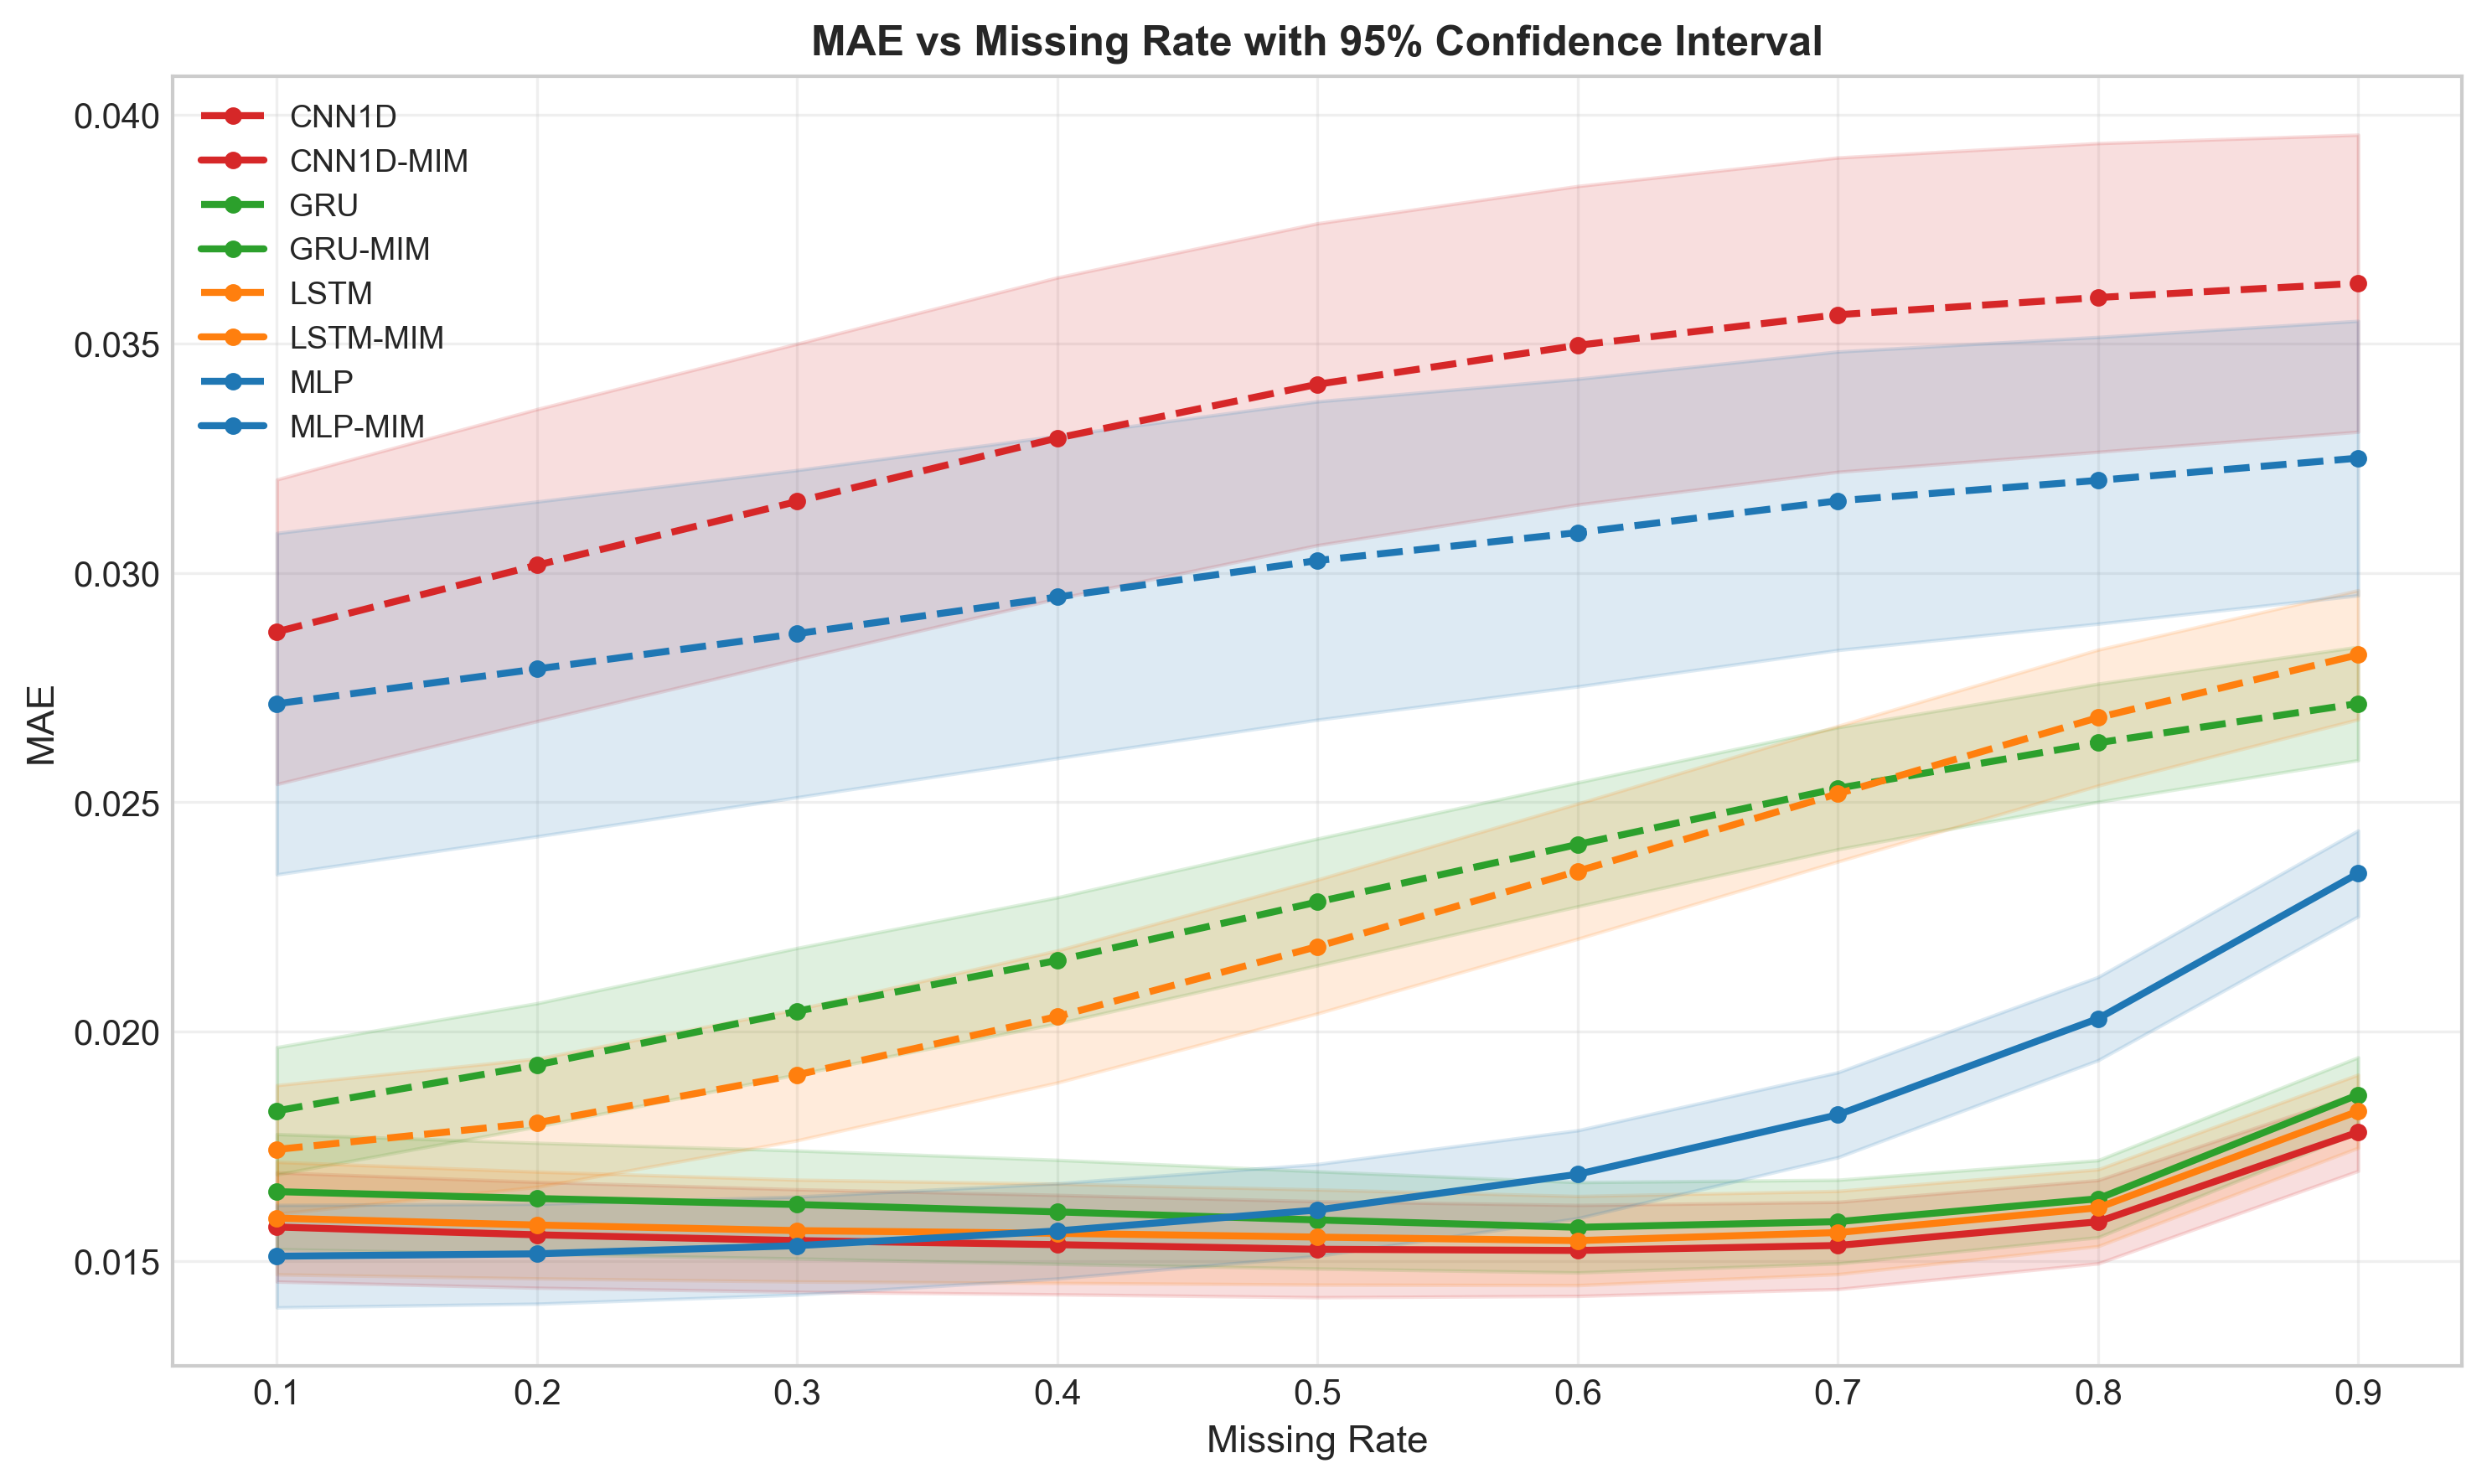
\includegraphics[width=0.48\textwidth]{mae_curves_ci.png}%
        \label{fig:mae_curves}%
    }%
    \hfill
    \subfloat[MAE heatmap (model $\times$ missing rate)]{%
        
\includegraphics[width=0.48\textwidth]{mae_heatmap.png}%
        \label{fig:mae_heatmap}%
    }%
    \caption{MAE performance comparison of different models under different missing rates. (a) MAE curves: solid lines for MIM, dashed lines for Baseline, shaded regions for 95\% confidence intervals; (b) Heatmap: upper part for Baseline, lower part for MIM, lighter colors indicate lower MAE.}
    \label{fig:mae_comparison}
\end{figure*}

Experimental data shows the following trends:

(1) \textbf{MAE increases monotonically with missing rate}: MAE of all models increases with MR, reflecting increased prediction difficulty as available information decreases.

(2) \textbf{MIM outperforms Baseline at all missing rates}: At MR=0.1, MAE improvement of MIM relative to Baseline is approximately 8.6\%--45.2\%; at MR=0.5, improvement increases to 26\%--57\% (1D-CNN-MIM improvement rate reaches 55.3\%, MLP-MIM is 46.8\%).

(3) \textbf{Advantages are more prominent under high missing rates}: At MR$\geq$0.7, Baseline MAE generally exceeds 0.032, while MIM versions remain below 0.023; at MR=0.9, Baseline MAE generally exceeds 0.029, while MIM versions remain below 0.029.

Table~\ref{tab:full_results} provides detailed numerical comparisons at four key missing rates (0.3, 0.5, 0.7, 0.9). Data indicates that MIM versions of all four deep learning models achieve lower MAE than corresponding Baseline versions under all tested missing rate conditions.

\begin{table*}[t]
\centering
\small
\caption{MAE Comparison and Improvement Rates Under Different Missing Rates (100 random seeds, mean$\pm$std, best values bolded)}
\label{tab:full_results}
\begin{tabular}{@{}llcccc@{}}
\toprule
\textbf{Model} & \textbf{Strategy} & \textbf{MR=0.3} & \textbf{MR=0.5} & \textbf{MR=0.7} & \textbf{MR=0.9} \\
\midrule
\multirow{3}{*}{MLP} 
& Baseline & 0.029$\pm$0.018 & 0.030$\pm$0.017 & 0.032$\pm$0.016 & 0.033$\pm$0.015 \\
& MIM & \textbf{0.015}$\pm$0.005 & \textbf{0.016}$\pm$0.005 & \textbf{0.018}$\pm$0.005 & \textbf{0.023}$\pm$0.005 \\
& Improvement & 46.5\% & 46.8\% & 42.4\% & 27.9\% \\
\midrule
\multirow{3}{*}{LSTM} 
& Baseline & 0.019$\pm$0.007 & 0.022$\pm$0.007 & 0.025$\pm$0.007 & 0.028$\pm$0.007 \\
& MIM & \textbf{0.016}$\pm$0.006 & \textbf{0.016}$\pm$0.005 & \textbf{0.016}$\pm$0.005 & \textbf{0.018}$\pm$0.004 \\
& Improvement & 17.8\% & 29.0\% & 38.0\% & 35.3\% \\
\midrule
\multirow{3}{*}{GRU} 
& Baseline & 0.020$\pm$0.007 & 0.023$\pm$0.007 & 0.025$\pm$0.007 & 0.027$\pm$0.006 \\
& MIM & \textbf{0.016}$\pm$0.006 & \textbf{0.016}$\pm$0.005 & \textbf{0.016}$\pm$0.005 & \textbf{0.019}$\pm$0.004 \\
& Improvement & 20.6\% & 30.4\% & 37.4\% & 31.4\% \\
\midrule
\multirow{3}{*}{1D-CNN} 
& Baseline & 0.032$\pm$0.017 & 0.034$\pm$0.018 & 0.036$\pm$0.017 & 0.036$\pm$0.016 \\
& MIM & \textbf{0.015}$\pm$0.006 & \textbf{0.015}$\pm$0.005 & \textbf{0.015}$\pm$0.005 & \textbf{0.018}$\pm$0.004 \\
& Improvement & 51.1\% & 55.3\% & 57.0\% & 51.0\% \\
\bottomrule
\end{tabular}
\end{table*}

\subsection{MIM Improvement Rate and Statistical Significance}

This section quantifies MIM performance benefits through statistical testing. The improvement rate is defined as:
\begin{equation}
    \text{Improvement}(\%) = \frac{\text{MAE}_{\text{Baseline}} - \text{MAE}_{\text{MIM}}}{\text{MAE}_{\text{Baseline}}} \times 100\%
\end{equation}

For each model--missing rate combination, 100 pairs of $(\text{MAE}_{\text{Baseline}}, \text{MAE}_{\text{MIM}})$ samples are obtained based on 100 random seeds. Wilcoxon signed-rank test (non-parametric) is used for paired comparison, with null hypothesis $H_0$ being ``at this missing rate, MIM and Baseline MAE distributions have no significant difference,'' and significance level $\alpha=0.05$.

Table~\ref{tab:improvement_summary} summarizes improvement rates for each model at key missing rate points. Data shows: at MR$\geq$0.4, improvement rates for all four models are significantly positive; 1D-CNN has the highest average improvement rate (52.6\%), while LSTM and GRU improvement rates increase monotonically with missing rate (increasing from 17.8\%/20.6\% at MR=0.3 to 38.0\%/37.4\% at MR=0.7).

\begin{table}[t]
\centering
\caption{Summary of MAE Improvement Rates of MIM vs Baseline (\%)}
\label{tab:improvement_summary}
\resizebox{\columnwidth}{!}{%
\begin{tabular}{@{}lcccccc@{}}
\toprule
\textbf{Model} & \textbf{0.1} & \textbf{0.3} & \textbf{0.5} & \textbf{0.7} & \textbf{0.9} & \textbf{Average} \\
\midrule
MLP & 44.4 & 46.5 & 46.8 & 42.4 & 27.9 & 42.5 \\
LSTM & 8.6 & 17.8 & 29.0 & 38.0 & 35.3 & 26.5 \\
GRU & 9.6 & 20.6 & 30.4 & 37.4 & 31.4 & 26.9 \\
1D-CNN & 45.2 & 51.1 & 55.3 & 57.0 & 51.0 & 52.6 \\
\bottomrule
\end{tabular}%
}
\end{table}

Figure~\ref{fig:improvement} shows the curves of improvement rates for each model varying with missing rate.

\begin{figure}[t]
    \centering
    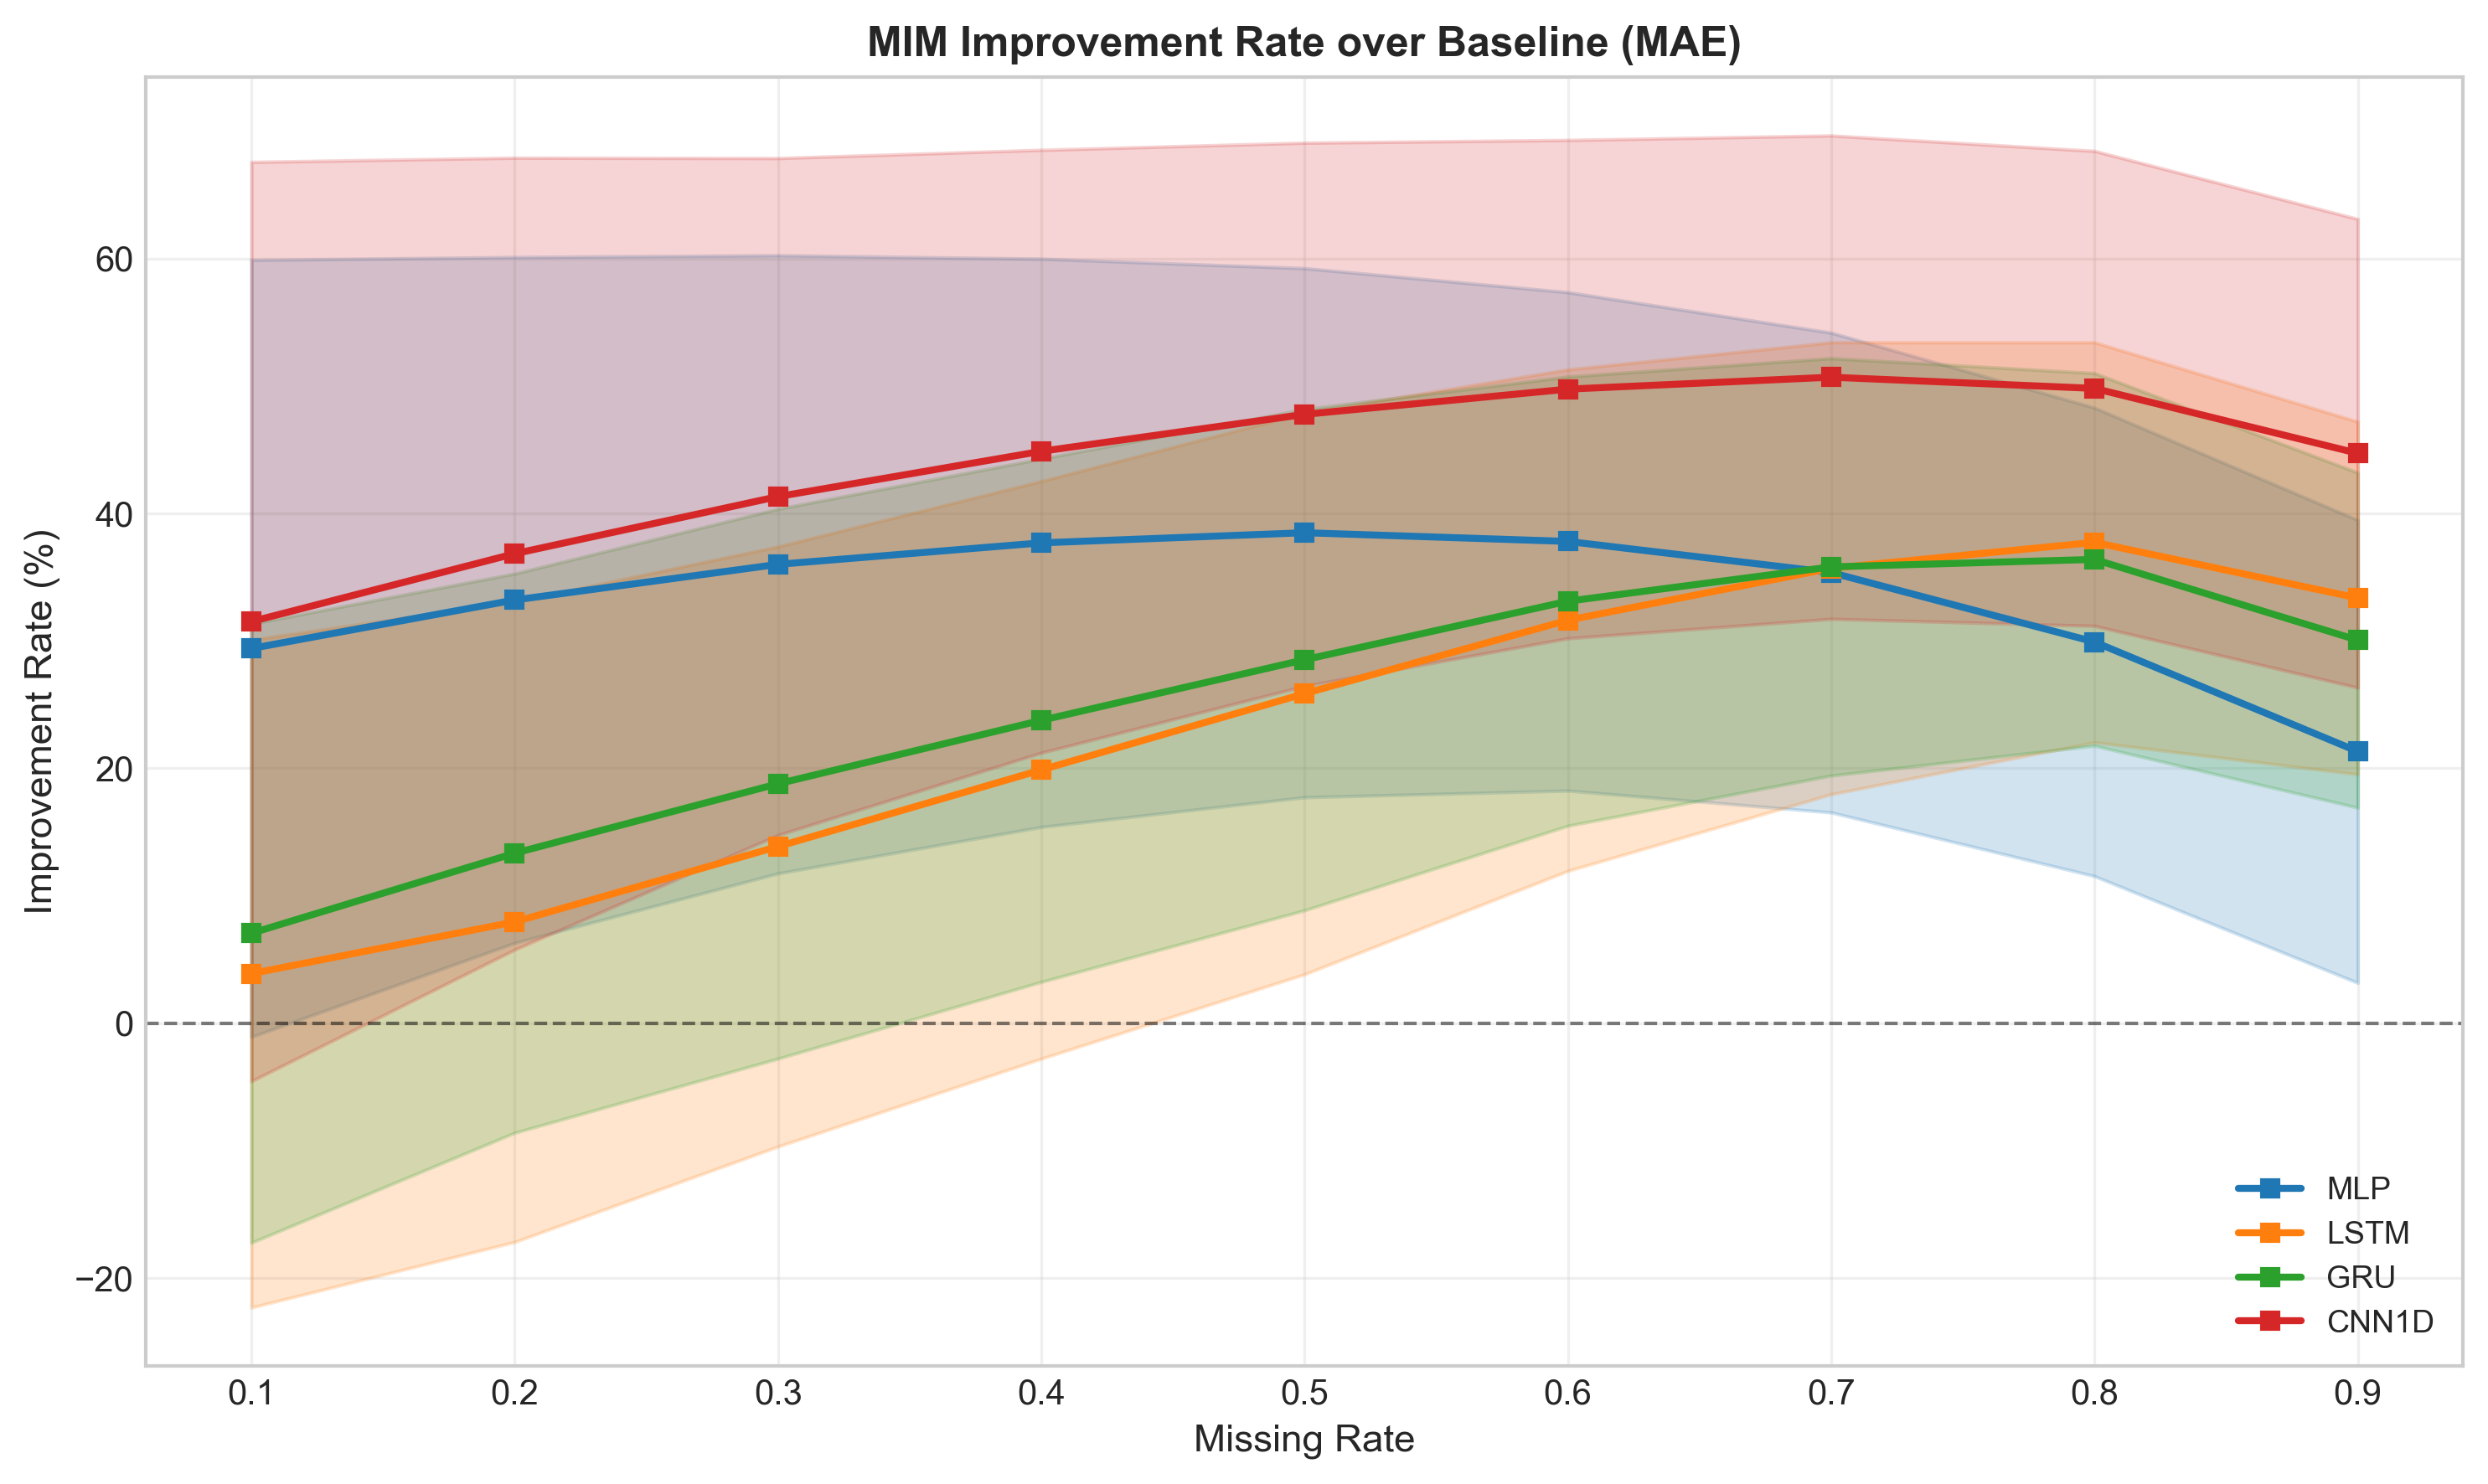
\includegraphics[width=\columnwidth]{mae_improvement_rate.png}
    \caption{MAE improvement rate curves of MIM vs Baseline varying with missing rate. Positive values indicate MIM outperforms Baseline.}
    \label{fig:improvement}
\end{figure}

Wilcoxon signed-rank test results (Table~\ref{tab:significance}) show: at $\alpha=0.05$ significance level, all model--MIM combinations have $p$-values less than 0.01 (the vast majority less than 0.001), indicating that performance improvements brought by MIM are statistically significant.

\begin{table}[t]
\centering
\small
\caption{Wilcoxon Signed-Rank Test Results (MIM vs Baseline)}
\label{tab:significance}
\begin{tabular}{@{}lcccc@{}}
\toprule
\textbf{Model} & \textbf{MR=0.3} & \textbf{MR=0.5} & \textbf{MR=0.7} & \textbf{MR=0.9} \\
\midrule
MLP & $<$0.001*** & $<$0.001*** & $<$0.001*** & 0.001** \\
LSTM & $<$0.001*** & $<$0.001*** & $<$0.001*** & $<$0.001*** \\
GRU & $<$0.001*** & $<$0.001*** & $<$0.001*** & $<$0.001*** \\
1D-CNN & $<$0.001*** & $<$0.001*** & $<$0.001*** & $<$0.001*** \\
\bottomrule
\end{tabular}
\\[3pt]
\footnotesize Note: *** indicates $p<$0.001, ** indicates $p<$0.01, Wilcoxon signed-rank test, two-tailed, $K=$100 random seeds.
\end{table}

\textbf{Seed stability analysis}: Figure~\ref{fig:seed_stability} shows MAE distributions across 100 random seeds. In the MR$\geq$0.4 range, MIM versions not only have lower means but also smaller standard deviations (e.g., at MR=0.5, MIM version standard deviation is approximately 0.005, Baseline approximately 0.007--0.018), indicating that the MIM strategy significantly reduces model sensitivity to random initialization and data partitioning.

\begin{figure}[t]
    \centering
    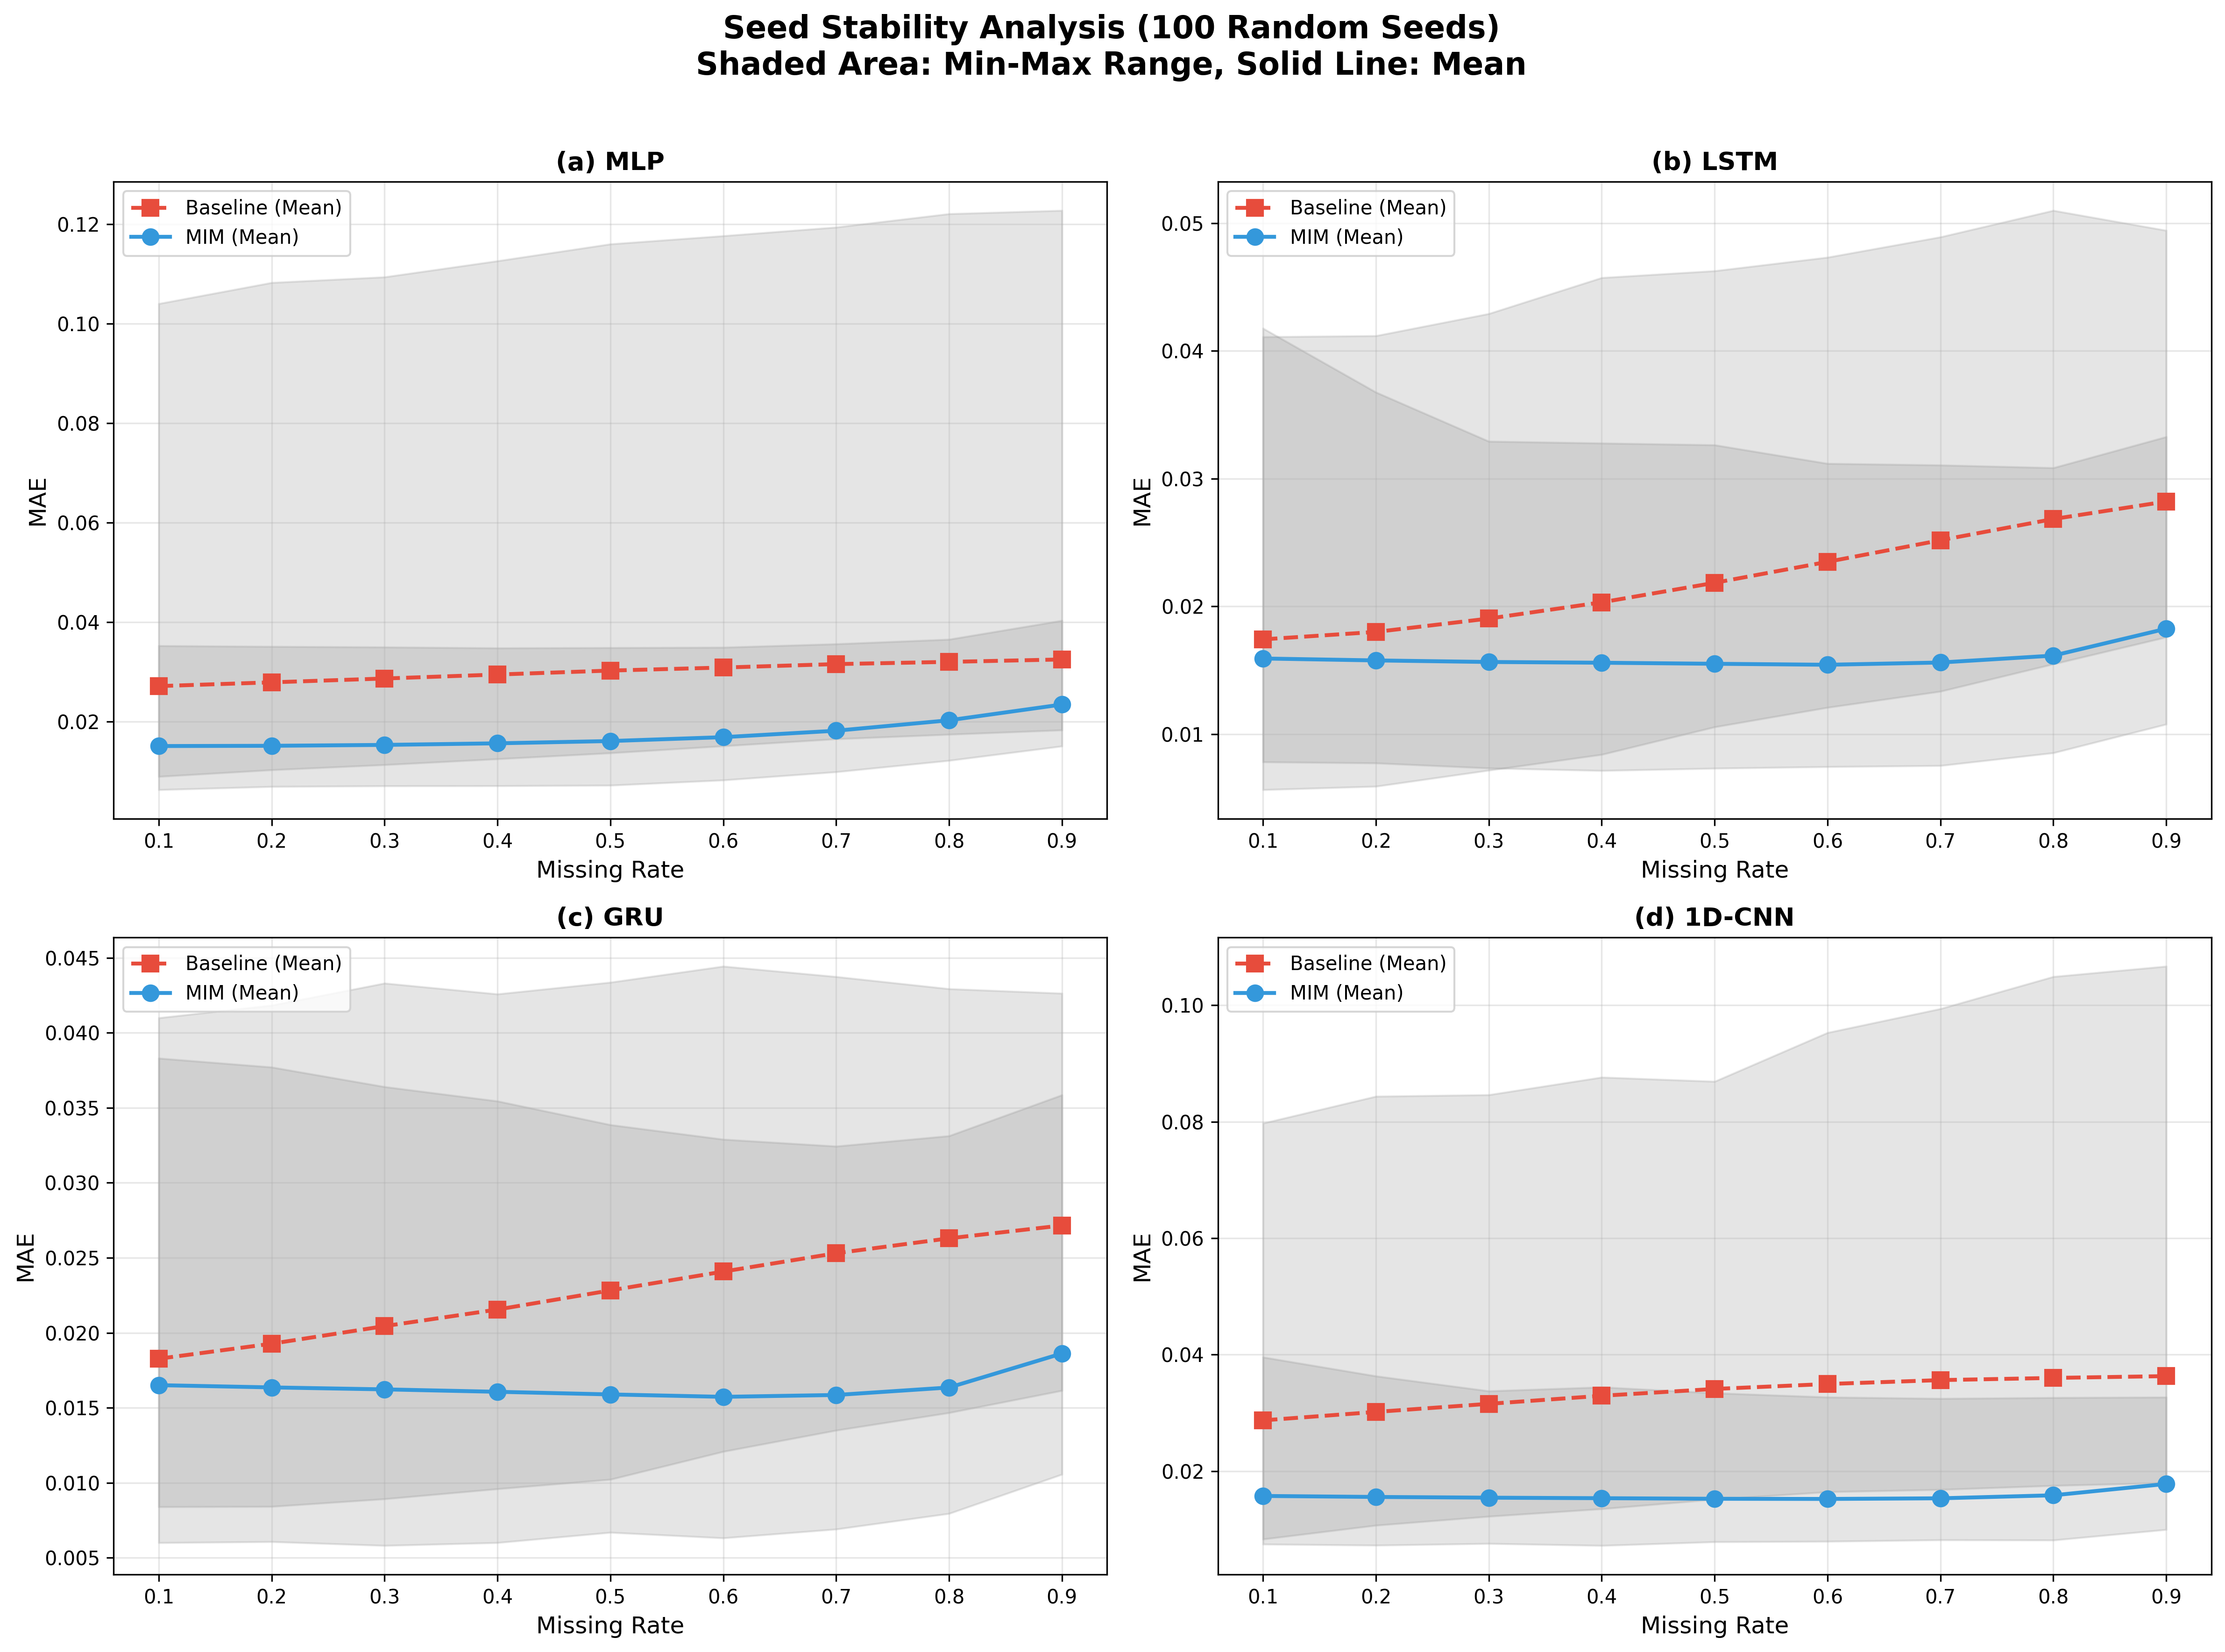
\includegraphics[width=\columnwidth]{fig9_seed_stability_v2.png}
    \caption{Seed stability analysis (100 random seeds). Gray shaded area represents min-max range, colored solid lines represent cross-seed means for MIM, dashed lines represent cross-seed means for Baseline.}
    \label{fig:seed_stability}
\end{figure}

\subsection{Architecture Differences and Extreme Missing Robustness}

This section analyzes research question RQ2 (architecture differences) and RQ3 (extreme missing robustness).

\textbf{Architecture differences}: Table~\ref{tab:improvement_summary} data shows that under medium-high missing rate (MR$\geq$0.5) conditions, MIM benefits vary among different architectures. 1D-CNN maintains high improvement rates across all missing rate intervals (45\%--57\%); LSTM and GRU improvement rates increase with missing rate.

\textbf{Extreme missing robustness}: Under extreme conditions at MR=0.9, model performances are shown in Table~\ref{tab:full_results}. The four ``model+MIM'' combinations maintain MAE between 0.018--0.023, achieving 27.9\%--51.0\% error reduction relative to Baseline (0.028--0.036). Among them, 1D-CNN-MIM performs best (MAE=0.018), followed by LSTM-MIM and GRU-MIM (MAE approximately 0.018--0.019), with MLP-MIM at 0.023.

The violin plot in Figure~\ref{fig:distribution} shows that as missing rate increases, Baseline model MAE distributions gradually shift rightward and broaden (increased dispersion), while MIM version distribution centers remain at low levels with more concentrated shapes.

\begin{figure*}[t]
    \centering
    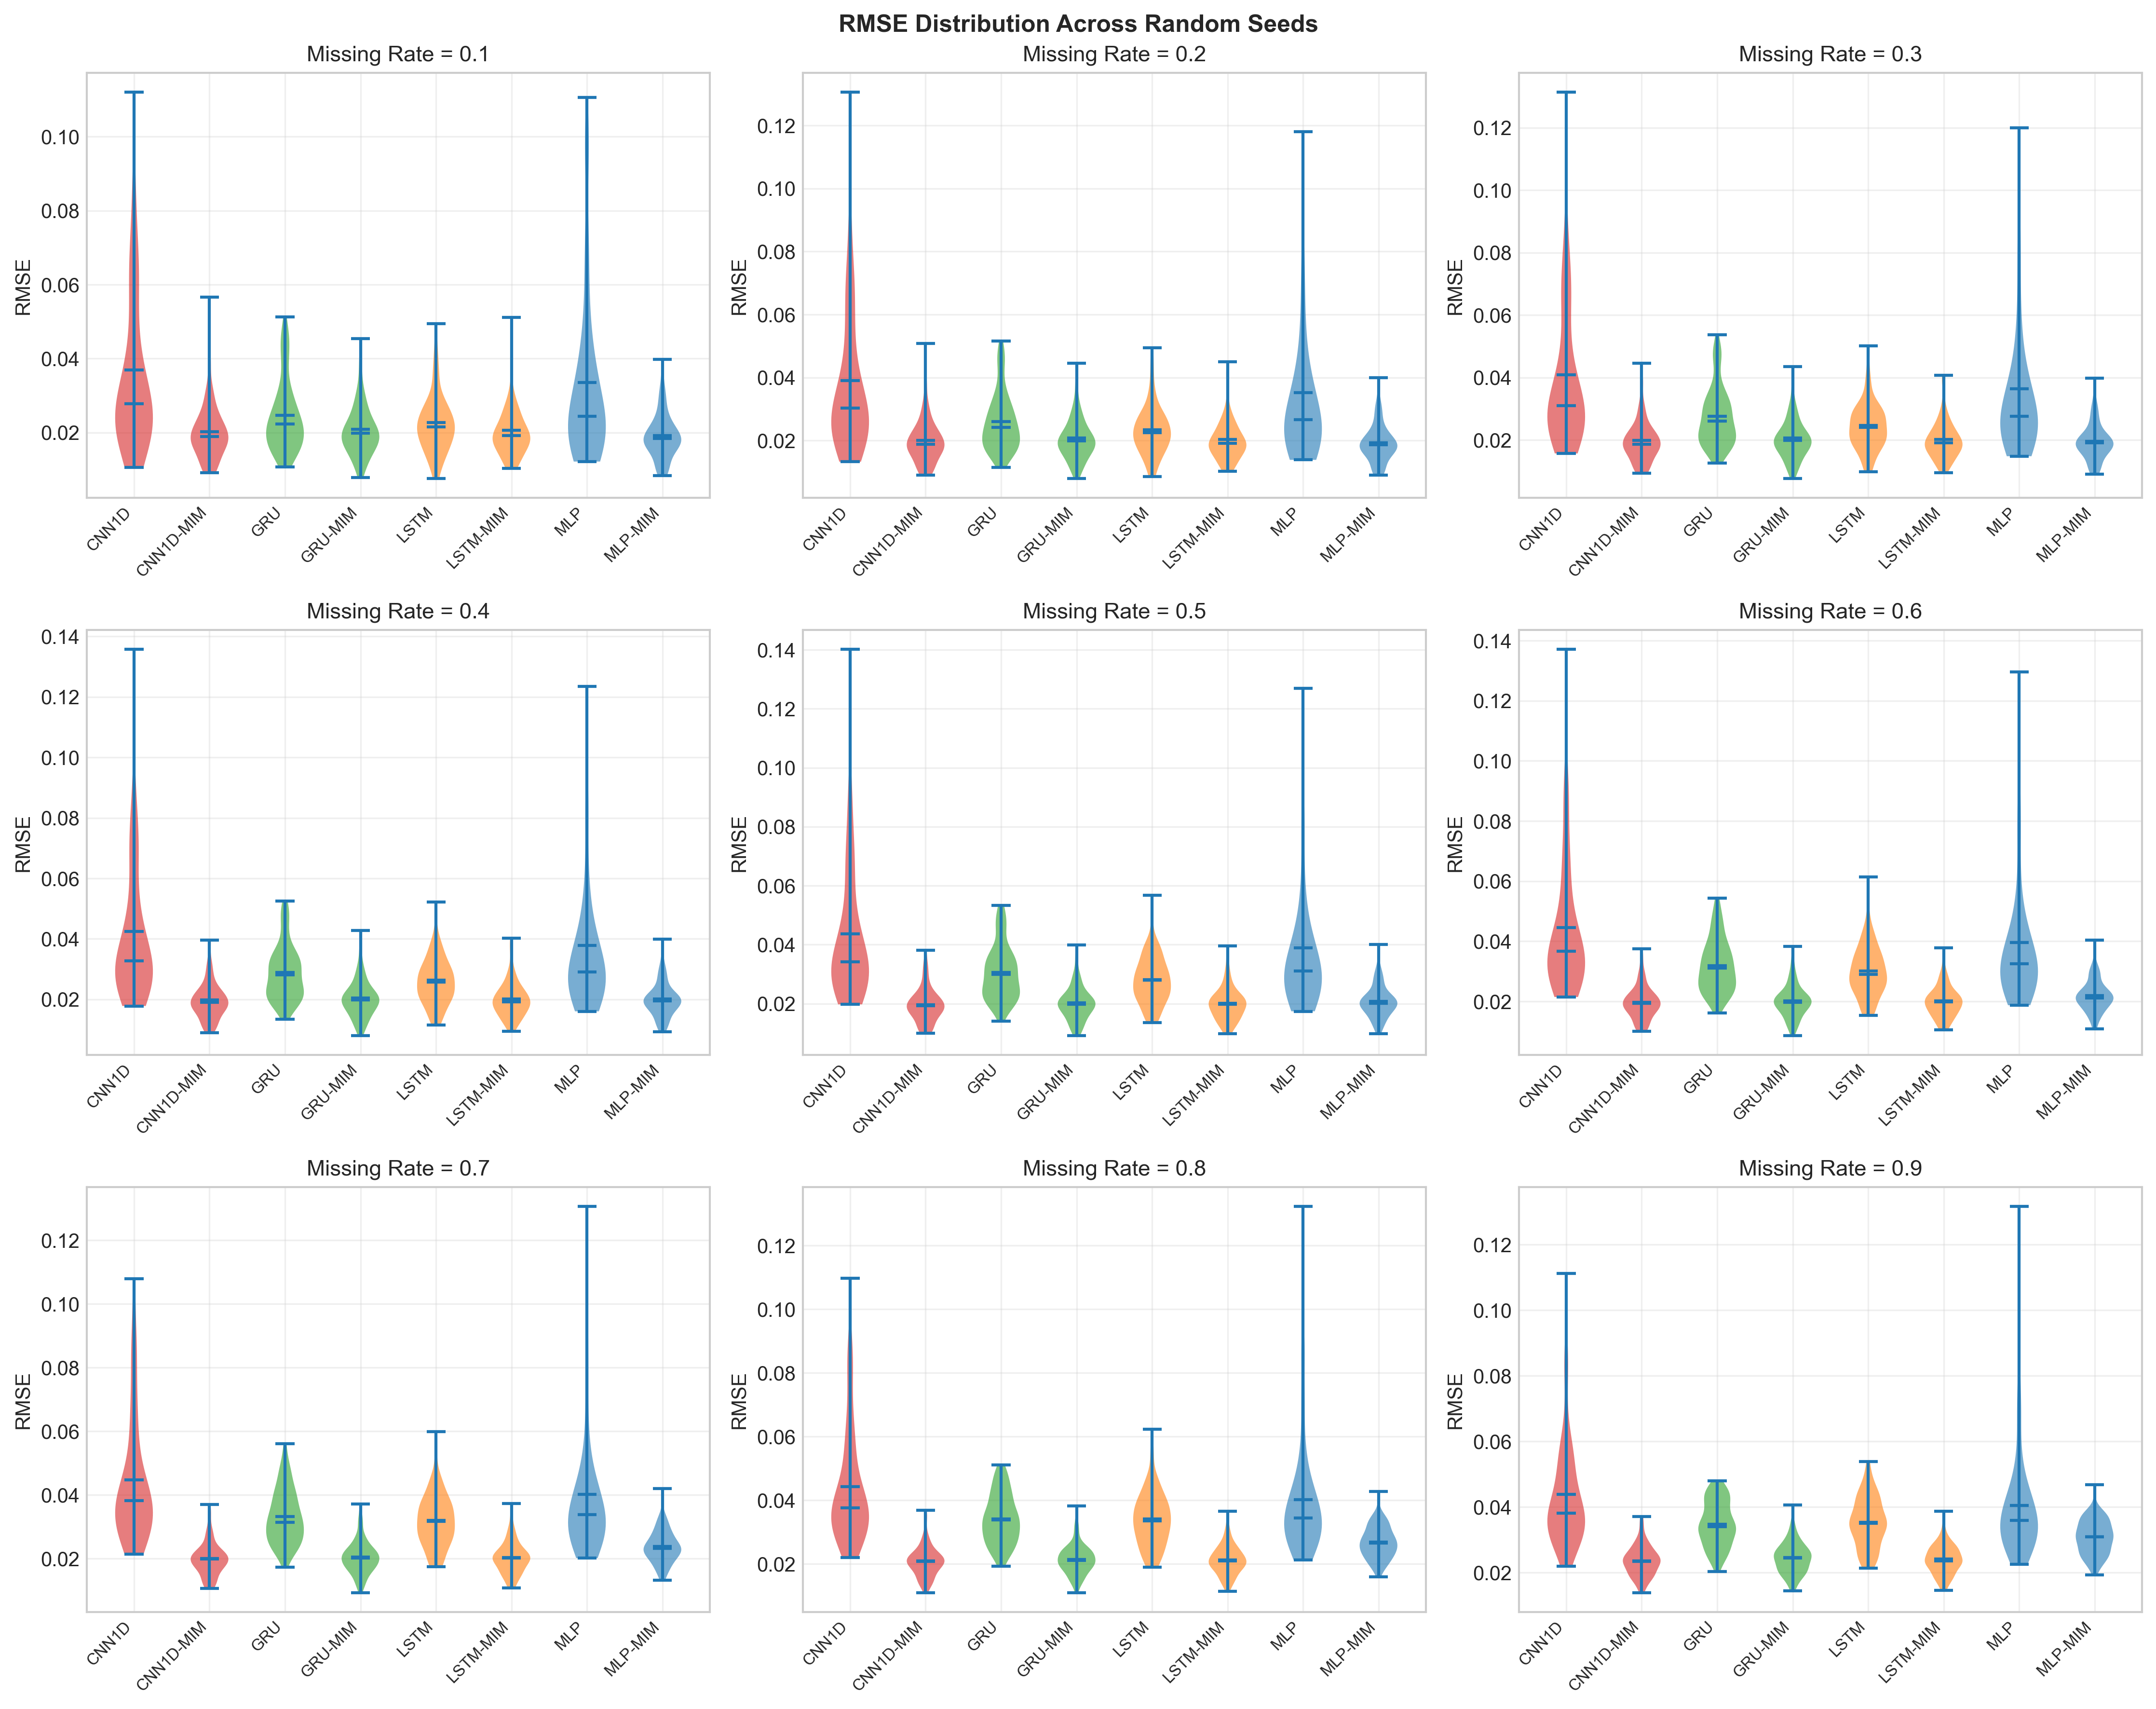
\includegraphics[width=\textwidth]{rmse_distribution.png}
    \caption{MAE distribution under different missing rates (violin plot).}
    \label{fig:distribution}
\end{figure*}

%==============================================================================

\section{Discussion and Implications for BMS}\label{sec:discussion}

\subsection{MIM Mechanism and Model Behavior Analysis}

Based on experimental results in Section~\ref{sec:results}, this section provides careful analysis of the MIM mechanism. In Section~\ref{sec:results}, experiments observed the following consistent phenomena: in the medium-high missing rate range of MR$\geq$0.4, MAE of all four deep learning architectures (MLP, LSTM, GRU, 1D-CNN) under MIM input strategy is significantly lower than corresponding Baseline versions, with improvement rates in the range of approximately 26\%--57\% (Table~\ref{tab:improvement_summary} and Figure~\ref{fig:mae_curves}). Under extreme missing conditions at MR=0.9, Baseline model MAE generally exceeds 0.028, while MIM combinations (MLP-MIM, LSTM-MIM, GRU-MIM, 1D-CNN-MIM) can still maintain low levels of 0.018--0.023 (Table~\ref{tab:full_results}). Wilcoxon signed-rank test $p$-values at key missing rates (MR=0.3, 0.5, 0.7, 0.9) are all significantly less than 0.05, with the vast majority less than 0.001 (Table~\ref{tab:significance}), indicating that improvements brought by MIM have statistical significance.

The above phenomena are consistent with the design of MIM explicitly encoding missing patterns as input. Traditional Baseline methods only receive the imputed feature matrix $\hat{X}$, unable to distinguish which elements are real observations and which are imputed estimates. In contrast, MIM explicitly marks the missing status of each feature position through the binary missing indicator matrix $M$, equivalent to providing the network with a ``reliability weighting'' signal. During training, neural networks can learn joint dependencies on ``observed values + missing labels,'' automatically reducing reliance on features with high missing rates and low confidence. Even under the MCAR assumption, explicitly distinguishing observations from imputations helps limit the propagation of imputation errors; while in practical scenarios closer to MAR or MNAR, missing patterns themselves may also carry indirect information related to SOH (such as correlations between certain sensor failures and battery aging states).

Different architectures exhibit significant differences in their degree of benefit from MIM. Table~\ref{tab:improvement_summary} shows that 1D-CNN maintains high improvement rates across the full range of MR=0.1--0.9 (45\%--57\%), with MAE dropping to 0.018 at MR=0.9 (Table~\ref{tab:full_results}). A possible reason is that 1D-CNN's local receptive field structure facilitates the utilization of local patterns along the feature dimension, while the $M$ mask helps convolution kernels focus on local regions with more real observations, reducing interference from imputation noise on convolution responses. LSTM and GRU improvement rates increase with missing rate at MR$\geq$0.5 (38\% and 31\% at MR=0.9 respectively); their temporal gating mechanisms may balance information from time slices with and without missing data along the temporal dimension, with missing indicators helping memory cells distinguish between ``credible'' and ``non-credible'' inputs. MLP shows obvious improvement at MR$\leq$0.6 (average approximately 46\%), but improvement decreases to 27.9\% at MR=0.9, possibly due to its lack of explicit temporal or local structure modeling capabilities---under extreme high missing rates, although MIM still provides missing position information, the fully connected structure struggles to effectively utilize this prior to reconstruct feature associations. It should be noted that the above mechanism explanations are only reasonable inferences based on experimental phenomena; more rigorous theoretical explanations still await future work through ablation experiments and interpretability analysis for verification.

\subsection{BMS-Oriented Model and Configuration Selection Recommendations}

Based on experimental results in Section~\ref{sec:results}, this section reconstructs engineering recommendations in tabular form (Table~\ref{tab:bms_selection}), facilitating quick reference and implementation by BMS engineers.

\begin{table*}[t]
\centering
\small
\caption{BMS-Oriented Model and MIM Selection Recommendations for Missing Rate Scenarios}
\label{tab:bms_selection}
\begin{tabular}{@{}p{2.5cm}p{4cm}p{6cm}@{}}
\toprule
\textbf{Missing Rate Interval} & \textbf{Recommended Architecture Combination} & \textbf{Engineering Notes} \\
\midrule
MR$\leq$0.3 & MLP-Baseline / MLP-MIM & \textbf{Complexity:} Low (parameter count approximately $3.1\times10^4$); \textbf{Applicable hardware:} Embedded BMS chips; \textbf{Scenario:} Single vehicles or small-scale energy storage units with good data quality; Baseline can be used when resources are extremely constrained, otherwise MLP-MIM is recommended as the default choice \\
\midrule
0.3$<$MR$\leq$0.6 & MLP-MIM / 1D-CNN-MIM & \textbf{Complexity:} Low--Medium (parameter count approximately $2.1\times10^4$--$3.1\times10^4$); \textbf{Applicable hardware:} Edge computing nodes, onboard processors; \textbf{Scenario:} Fleet monitoring or energy storage stations with medium missing rates (MR), improvement rates of 46\%--55\% at MR=0.5 (Table~\ref{tab:improvement_summary}) \\
\midrule
MR$\geq$0.7 & 1D-CNN-MIM / LSTM-MIM & \textbf{Complexity:} Medium (parameter count approximately $2.1\times10^4$--$3.5\times10^4$); \textbf{Applicable hardware:} Fleet cloud/energy storage station servers; \textbf{Scenario:} High missing rate or frequent sensor failure conditions, MIM versions maintain MAE at 0.018--0.019 at MR=0.9 (Table~\ref{tab:full_results}) \\
\bottomrule
\end{tabular}
\end{table*}

In the low missing rate range (MR$\leq$0.3), Baseline models can already achieve good prediction performance (MAE approximately 0.027 at MR=0.1, Table~\ref{tab:full_results}). In this range, introducing MIM can further reduce errors (to approximately 0.015), but relative benefits are limited. Therefore, in embedded BMS chip scenarios with extremely limited computational resources, MLP-Baseline can be prioritized; if there is some margin for accuracy requirements, MLP-MIM is recommended as the default configuration.

In the medium missing rate range (0.3$<$MR$\leq$0.6), missing data begins to significantly affect Baseline performance, while MIM benefits become apparent. Taking MR=0.5 as an example, MLP-MIM reduces MAE from 0.030 to 0.016, and 1D-CNN-MIM from 0.034 to 0.015 (Table~\ref{tab:full_results}), with improvement rates reaching 46.8\% and 55.3\% respectively (Table~\ref{tab:improvement_summary}). The two represent ``lightweight efficient solution'' and ``performance-prioritized solution'' respectively, suitable as general deployment choices for fleet-level monitoring or energy storage station edge nodes.

In the high missing rate range (MR$\geq$0.7), without using MIM, errors and instability increase significantly (Baseline MAE reaches 0.028--0.036 at MR=0.9). At this point, 1D-CNN-MIM or LSTM-MIM are recommended: the former achieves MAE of only 0.018 at MR=0.9 with 51.0\% improvement rate; the latter achieves MAE of approximately 0.018--0.019 with 38.0\%--42.1\% improvement rate (Table~\ref{tab:full_results}). These two architectures are suitable for deployment on fleet cloud or grid-scale energy storage station servers, capable of maintaining usable SOH prediction accuracy under high-frequency sensor failure conditions.

Regarding inference complexity and real-time performance: based on parameter count estimates given in Section~\ref{sec:method}, MLP-MIM has a parameter scale of approximately $\mathcal{O}(10^4)$ order of magnitude, with forward inference requiring only matrix multiplication and activation operations, suitable for real-time SOH prediction on resource-constrained embedded BMS. 1D-CNN-MIM and LSTM-MIM have slightly higher parameter counts (approximately $2\times10^4$--$4\times10^4$) and involve convolutional or temporal recurrent computations, but their computational overhead remains within acceptable range when inferring on fleet cloud or grid-scale energy storage station servers. In actual deployment, model configurations can be selected from the recommended architecture combinations in Table~\ref{tab:bms_selection} according to target hardware computational power and storage budget.

\subsection{Research Boundaries and Future Extension Directions}

Although this study systematically evaluated the MIM method under multi-model and multi-missing-rate conditions, there are still several boundaries and limitations. The following analyzes these limitations and their impact on result interpretation from three dimensions, and provides targeted future work directions.

\textbf{Limitation 1: Missing mechanisms.} Current experiments only consider missing completely at random (MCAR), without systematic evaluation under MAR (missing at random) or MNAR (missing not at random) scenarios closer to reality. In real fleet and grid-scale energy storage data, missing data is often influenced by operating conditions, aging, and maintenance strategies---for example, batteries with higher aging degrees may be more prone to sensor failures, causing missing data to be correlated with SOH itself. The MCAR assumption in this paper may underestimate or misestimate MIM benefits in real scenarios: if missing data is correlated with SOH (MAR/MNAR), missing pattern $M$ may carry more information related to the target variable, and MIM's potential value may be higher; conversely, if missing mechanisms have complex interactions with existing features, the simple concatenation strategy of $[\hat{X}|M]$ may require adjustment.

\textit{Future direction:} Annotate missing causes (such as sensor failure codes, communication logs) on actual BMS collected data, constructing more realistic MAR/MNAR missing mechanism assumptions; compare MIM with methods explicitly modeling missing mechanisms (such as mask-based temporal models, generative missing modeling) under these scenarios, systematically characterizing MIM's applicable boundaries.

\textbf{Limitation 2: Dataset and task scope.} This study only uses the single XJTU dataset and single SOH regression task for validation. The generalizability and applicability of results remain limited, and cannot be directly extrapolated to other publicly available datasets such as NASA, CALCE, Oxford, or other battery health management tasks such as remaining useful life (RUL) prediction and fault diagnosis. Different datasets have varying collection conditions, battery chemistries, and operating condition distributions; the effectiveness of MIM strategies in these scenarios requires independent validation.

\textit{Future direction:} Reproduce experiments on multiple datasets (NASA, CALCE, Oxford, etc.) and multiple tasks (SOH/RUL/anomaly detection) to verify the generalizability of the ``missing as signal'' paradigm; study the combination of MIM with Domain Adaptation methods for data distribution shift problems that may exist in actual BMS.

\textbf{Limitation 3: Imputation strategies and model families.} This paper only adopts mean imputation as the unified baseline, and models only cover four classical architectures: MLP, LSTM, GRU, and 1D-CNN. Systematic comparison between ``improvement space of imputation methods'' and ``whether to adopt MIM'' relative importance has not been conducted, nor have benefits and costs of more complex attention architectures (such as Transformer) been evaluated. If more complex imputation methods (such as KNN, iterative imputation, generative models) are adopted, Baseline performance may improve, and MIM's relative improvement magnitude may change.

\textit{Future direction:} Introduce various imputation methods (KNN, regression imputation, matrix factorization, generative models, etc.) and compare them in combination with MIM, verifying whether ``MIM + simple imputation'' is sufficient to match complex imputation strategies; explore the combination of MIM with emerging architectures such as Transformer and Graph Neural Networks (GNN), while quantifying their computational power and power consumption overhead in BMS scenarios to evaluate engineering feasibility.

As electric vehicle fleets and grid-scale energy storage systems continue to expand in scale, the need to maintain SOH prediction robustness under missing data conditions becomes increasingly important. This paper conducted systematic empirical research around the ``missing as signal'' paradigm; future work still needs to advance in real BMS data, physics model fusion, and dispatch/maintenance coordinated decision-making to truly support the safe and efficient operation of energy systems.

%==============================================================================
\section{Conclusion and Future Work}\label{sec:conclusion}

This paper conducts research on battery SOH prediction problems under data missing conditions, adopting the ``missing as signal'' MIM paradigm. Based on the XJTU publicly available lithium battery dataset, this paper constructs cycle-level sample units, designs MCAR missing simulations for nine levels of Missing Rate (MR) from 0.1--0.9, and conducts systematic evaluation of four typical deep learning architectures (MLP, LSTM, GRU, 1D-CNN) under multi-missing-rate and multi-random-seed conditions. Experimental results indicate that under medium-high missing rate (MR$\geq$0.4) conditions, MIM achieves significant performance improvements compared to imputation-only Baseline in metrics such as MAE, RMSE, and R\textsuperscript{2}, with particularly notable benefits for architectures such as 1D-CNN, and validated by statistical methods such as Wilcoxon signed-rank tests. This work provides systematic empirical evidence and a reproducible evaluation framework for research on explicitly encoding missing patterns in battery SOH prediction.

In practical application scenarios such as electric vehicle fleets and grid-scale energy storage systems, BMS needs to continuously estimate SOH under imperfect data conditions such as sensor failures and communication packet loss; the results of this paper provide empirical evidence for model and input strategy selection in such scenarios. In fleet applications, deep models adopting MIM (particularly 1D-CNN and LSTM architectures) can maintain more robust SOH estimation under medium-high missing rates, helping reduce health state misjudgment risks and optimize charging strategy and maintenance scheduling decisions. In grid-scale energy storage stations, long-term operation, sensor aging, and complex operating conditions make data missing more common; this study shows that reasonable selection of ``model+MIM'' combinations can significantly suppress prediction errors and instability under high missing rate conditions, providing more reliable health information support for frequency regulation, peak shaving and valley filling, and other services. The above findings have direct reference value for BMS software algorithm design and hardware computational power configuration, potentially improving battery asset utilization efficiency and operational safety.

Future research still has several directions worth exploring. This study was mainly completed under the MCAR missing setting; future work is needed to systematically evaluate and compare under MAR/MNAR mechanisms (missing data correlated with operating conditions, aging, and maintenance strategies) closer to actual BMS scenarios. Meanwhile, validating the generalizability and boundaries of the ``missing as signal'' paradigm on multiple publicly available datasets (NASA, CALCE, Oxford, etc.) and richer tasks (RUL prediction, anomaly detection, multi-task learning, etc.) is an important follow-up direction. Additionally, combining MIM with Transformer, Graph Neural Networks, and physics-informed model fusion methods, and systematically analyzing their computational power and power consumption costs in actual BMS deployment, also holds research value. Deep coupling of explicit missing modeling with decision systems such as fleet dispatch optimization and grid-scale energy storage participation in electricity markets is a key direction for promoting the system-level value of missing-robust SOH prediction.

%==============================================================================
\section*{Acknowledgments}

This work was supported by the Shandong Provincial Technology Innovation Guidance Program (Central Government Guides Local Science and Technology Development Funds) under Grant YDZX2024105.

%==============================================================================
\bibliographystyle{elsarticle-num}
\bibliography{references}

%==============================================================================

\end{document}
